\documentclass[]{book}
\usepackage{lmodern}
\usepackage{amssymb,amsmath}
\usepackage{ifxetex,ifluatex}
\usepackage{fixltx2e} % provides \textsubscript
\ifnum 0\ifxetex 1\fi\ifluatex 1\fi=0 % if pdftex
  \usepackage[T1]{fontenc}
  \usepackage[utf8]{inputenc}
\else % if luatex or xelatex
  \ifxetex
    \usepackage{mathspec}
  \else
    \usepackage{fontspec}
  \fi
  \defaultfontfeatures{Ligatures=TeX,Scale=MatchLowercase}
\fi
% use upquote if available, for straight quotes in verbatim environments
\IfFileExists{upquote.sty}{\usepackage{upquote}}{}
% use microtype if available
\IfFileExists{microtype.sty}{%
\usepackage{microtype}
\UseMicrotypeSet[protrusion]{basicmath} % disable protrusion for tt fonts
}{}
\usepackage[margin=1in]{geometry}
\usepackage{hyperref}
\hypersetup{unicode=true,
            pdftitle={Data Wrangling with R},
            pdfauthor={Claudia A Engel},
            pdfborder={0 0 0},
            breaklinks=true}
\urlstyle{same}  % don't use monospace font for urls
\usepackage{natbib}
\bibliographystyle{apalike}
\usepackage{color}
\usepackage{fancyvrb}
\newcommand{\VerbBar}{|}
\newcommand{\VERB}{\Verb[commandchars=\\\{\}]}
\DefineVerbatimEnvironment{Highlighting}{Verbatim}{commandchars=\\\{\}}
% Add ',fontsize=\small' for more characters per line
\usepackage{framed}
\definecolor{shadecolor}{RGB}{248,248,248}
\newenvironment{Shaded}{\begin{snugshade}}{\end{snugshade}}
\newcommand{\KeywordTok}[1]{\textcolor[rgb]{0.13,0.29,0.53}{\textbf{#1}}}
\newcommand{\DataTypeTok}[1]{\textcolor[rgb]{0.13,0.29,0.53}{#1}}
\newcommand{\DecValTok}[1]{\textcolor[rgb]{0.00,0.00,0.81}{#1}}
\newcommand{\BaseNTok}[1]{\textcolor[rgb]{0.00,0.00,0.81}{#1}}
\newcommand{\FloatTok}[1]{\textcolor[rgb]{0.00,0.00,0.81}{#1}}
\newcommand{\ConstantTok}[1]{\textcolor[rgb]{0.00,0.00,0.00}{#1}}
\newcommand{\CharTok}[1]{\textcolor[rgb]{0.31,0.60,0.02}{#1}}
\newcommand{\SpecialCharTok}[1]{\textcolor[rgb]{0.00,0.00,0.00}{#1}}
\newcommand{\StringTok}[1]{\textcolor[rgb]{0.31,0.60,0.02}{#1}}
\newcommand{\VerbatimStringTok}[1]{\textcolor[rgb]{0.31,0.60,0.02}{#1}}
\newcommand{\SpecialStringTok}[1]{\textcolor[rgb]{0.31,0.60,0.02}{#1}}
\newcommand{\ImportTok}[1]{#1}
\newcommand{\CommentTok}[1]{\textcolor[rgb]{0.56,0.35,0.01}{\textit{#1}}}
\newcommand{\DocumentationTok}[1]{\textcolor[rgb]{0.56,0.35,0.01}{\textbf{\textit{#1}}}}
\newcommand{\AnnotationTok}[1]{\textcolor[rgb]{0.56,0.35,0.01}{\textbf{\textit{#1}}}}
\newcommand{\CommentVarTok}[1]{\textcolor[rgb]{0.56,0.35,0.01}{\textbf{\textit{#1}}}}
\newcommand{\OtherTok}[1]{\textcolor[rgb]{0.56,0.35,0.01}{#1}}
\newcommand{\FunctionTok}[1]{\textcolor[rgb]{0.00,0.00,0.00}{#1}}
\newcommand{\VariableTok}[1]{\textcolor[rgb]{0.00,0.00,0.00}{#1}}
\newcommand{\ControlFlowTok}[1]{\textcolor[rgb]{0.13,0.29,0.53}{\textbf{#1}}}
\newcommand{\OperatorTok}[1]{\textcolor[rgb]{0.81,0.36,0.00}{\textbf{#1}}}
\newcommand{\BuiltInTok}[1]{#1}
\newcommand{\ExtensionTok}[1]{#1}
\newcommand{\PreprocessorTok}[1]{\textcolor[rgb]{0.56,0.35,0.01}{\textit{#1}}}
\newcommand{\AttributeTok}[1]{\textcolor[rgb]{0.77,0.63,0.00}{#1}}
\newcommand{\RegionMarkerTok}[1]{#1}
\newcommand{\InformationTok}[1]{\textcolor[rgb]{0.56,0.35,0.01}{\textbf{\textit{#1}}}}
\newcommand{\WarningTok}[1]{\textcolor[rgb]{0.56,0.35,0.01}{\textbf{\textit{#1}}}}
\newcommand{\AlertTok}[1]{\textcolor[rgb]{0.94,0.16,0.16}{#1}}
\newcommand{\ErrorTok}[1]{\textcolor[rgb]{0.64,0.00,0.00}{\textbf{#1}}}
\newcommand{\NormalTok}[1]{#1}
\usepackage{longtable,booktabs}
\usepackage{graphicx,grffile}
\makeatletter
\def\maxwidth{\ifdim\Gin@nat@width>\linewidth\linewidth\else\Gin@nat@width\fi}
\def\maxheight{\ifdim\Gin@nat@height>\textheight\textheight\else\Gin@nat@height\fi}
\makeatother
% Scale images if necessary, so that they will not overflow the page
% margins by default, and it is still possible to overwrite the defaults
% using explicit options in \includegraphics[width, height, ...]{}
\setkeys{Gin}{width=\maxwidth,height=\maxheight,keepaspectratio}
\IfFileExists{parskip.sty}{%
\usepackage{parskip}
}{% else
\setlength{\parindent}{0pt}
\setlength{\parskip}{6pt plus 2pt minus 1pt}
}
\setlength{\emergencystretch}{3em}  % prevent overfull lines
\providecommand{\tightlist}{%
  \setlength{\itemsep}{0pt}\setlength{\parskip}{0pt}}
\setcounter{secnumdepth}{5}
% Redefines (sub)paragraphs to behave more like sections
\ifx\paragraph\undefined\else
\let\oldparagraph\paragraph
\renewcommand{\paragraph}[1]{\oldparagraph{#1}\mbox{}}
\fi
\ifx\subparagraph\undefined\else
\let\oldsubparagraph\subparagraph
\renewcommand{\subparagraph}[1]{\oldsubparagraph{#1}\mbox{}}
\fi

%%% Use protect on footnotes to avoid problems with footnotes in titles
\let\rmarkdownfootnote\footnote%
\def\footnote{\protect\rmarkdownfootnote}

%%% Change title format to be more compact
\usepackage{titling}

% Create subtitle command for use in maketitle
\newcommand{\subtitle}[1]{
  \posttitle{
    \begin{center}\large#1\end{center}
    }
}

\setlength{\droptitle}{-2em}

  \title{Data Wrangling with R}
    \pretitle{\vspace{\droptitle}\centering\huge}
  \posttitle{\par}
    \author{Claudia A Engel}
    \preauthor{\centering\large\emph}
  \postauthor{\par}
      \predate{\centering\large\emph}
  \postdate{\par}
    \date{Last updated: October 16, 2018}

\usepackage{booktabs}
\usepackage{amsthm}
\makeatletter
\def\thm@space@setup{%
  \thm@preskip=8pt plus 2pt minus 4pt
  \thm@postskip=\thm@preskip
}
\makeatother

\usepackage{amsthm}
\newtheorem{theorem}{Theorem}[chapter]
\newtheorem{lemma}{Lemma}[chapter]
\theoremstyle{definition}
\newtheorem{definition}{Definition}[chapter]
\newtheorem{corollary}{Corollary}[chapter]
\newtheorem{proposition}{Proposition}[chapter]
\theoremstyle{definition}
\newtheorem{example}{Example}[chapter]
\theoremstyle{definition}
\newtheorem{exercise}{Exercise}[chapter]
\theoremstyle{remark}
\newtheorem*{remark}{Remark}
\newtheorem*{solution}{Solution}
\begin{document}
\maketitle

{
\setcounter{tocdepth}{1}
\tableofcontents
}
\chapter*{Prerequisites and
Preparations}\label{prerequisites-and-preparations}
\addcontentsline{toc}{chapter}{Prerequisites and Preparations}

\begin{itemize}
\tightlist
\item
  You should have some \textbf{basic knowledge} of R, and be familiar
  with the topics covered in the
  \href{https://cengel.github.io/R-intro/}{Introduction to R}.
\item
  Have a recent version of \href{https://cran.r-project.org/}{R} and
  \href{https://www.rstudio.com/}{RStudio} installed.
\item
  Install and load the \texttt{tidyverse} package.
\end{itemize}

\begin{Shaded}
\begin{Highlighting}[]
\KeywordTok{install.packages}\NormalTok{(}\StringTok{"tidyverse"}\NormalTok{)  }
\KeywordTok{library}\NormalTok{(tidyverse)}
\end{Highlighting}
\end{Shaded}

\begin{itemize}
\tightlist
\item
  Create a new RStudio project \texttt{R-data-ws} in a new folder
  \texttt{R-data-ws}. Download both CSV files into a subdirectory called
  \texttt{data} like this:
\item
  Download \texttt{MS\_trafficstops\_bw\_age.csv}:
\end{itemize}

\begin{Shaded}
\begin{Highlighting}[]
\KeywordTok{download.file}\NormalTok{(}\StringTok{"https://github.com/cengel/R-data-wrangling/raw/master/data/MS_trafficstops_bw_age.csv"}\NormalTok{,}
              \StringTok{"data/MS_trafficstops_bw_age.csv"}\NormalTok{)}
\end{Highlighting}
\end{Shaded}

\begin{itemize}
\tightlist
\item
  Download \texttt{MS\_acs2015\_bw.csv}:
\end{itemize}

\begin{Shaded}
\begin{Highlighting}[]
\KeywordTok{download.file}\NormalTok{(}\StringTok{"https://github.com/cengel/R-data-wrangling/raw/master/data/MS_acs2015_bw.csv"}\NormalTok{,}
              \StringTok{"data/MS_acs2015_bw.csv"}\NormalTok{)}
\end{Highlighting}
\end{Shaded}

\section*{References}\label{references}
\addcontentsline{toc}{section}{References}

Boehmke, Bradley C. (2016) Data Wrangling with R
\url{http://link.springer.com/book/10.1007\%2F978-3-319-45599-0}

Grolemund, G \& Wickham, H (2017): R for Data Science
\url{http://r4ds.had.co.nz}

Wickham, H. (2014): Tidy Data
\url{https://www.jstatsoft.org/article/view/v059i10}

\section*{Acknowledgements}\label{acknowledgements}
\addcontentsline{toc}{section}{Acknowledgements}

Part of the materials for this tutorial are adapted from
\url{http://datacarpentry.org} and \url{http://softwarecarpentry.org}.

\chapter{\texorpdfstring{Data Manipulation using
\textbf{\texttt{dplyr}}}{Data Manipulation using dplyr}}\label{dplyr}

\begin{quote}
Learning Objectives

\begin{itemize}
\tightlist
\item
  Select columns in a data frame with the \textbf{\texttt{dplyr}}
  function \texttt{select}.
\item
  Select rows in a data frame according to filtering conditions with the
  \textbf{\texttt{dplyr}} function \texttt{filter}.
\item
  Direct the output of one \textbf{\texttt{dplyr}} function to the input
  of another function with the `pipe' operator
  \texttt{\%\textgreater{}\%}.
\item
  Add new columns to a data frame that are functions of existing columns
  with \texttt{mutate}.
\item
  Understand the split-apply-combine concept for data analysis.
\item
  Use \texttt{summarize}, \texttt{group\_by}, and \texttt{tally} to
  split a data frame into groups of observations, apply a summary
  statistics for each group, and then combine the results.
\end{itemize}
\end{quote}

\begin{center}\rule{0.5\linewidth}{\linethickness}\end{center}

We will be working a small subset of the data from the
\href{https://openpolicing.stanford.edu}{Stanford Open Policing
Project}. It contains information about traffic stops for blacks and
whites in the state of Mississippi during January 2013 to mid-July of
2016.

Let's begin with loading our sample data into a data frame.

\begin{Shaded}
\begin{Highlighting}[]
\NormalTok{trafficstops <-}\StringTok{ }\KeywordTok{read.csv}\NormalTok{(}\StringTok{"data/MS_trafficstops_bw_age.csv"}\NormalTok{)}
\end{Highlighting}
\end{Shaded}

Manipulation of dataframes is a common task when you start exploring
your data. We might select certain observations (rows) or variables
(columns), group the data by a certain variable(s), or calculate summary
statistics.

If we were interested in the mean age of the driver in different
counties we can do this using the normal base R operations:

\begin{Shaded}
\begin{Highlighting}[]
\KeywordTok{mean}\NormalTok{(trafficstops[trafficstops}\OperatorTok{$}\NormalTok{county_name }\OperatorTok{==}\StringTok{ "Tallahatchie County"}\NormalTok{, }\StringTok{"driver_age"}\NormalTok{], }\DataTypeTok{na.rm =} \OtherTok{TRUE}\NormalTok{)}
\end{Highlighting}
\end{Shaded}

\begin{verbatim}
#> [1] 36.70663
\end{verbatim}

\begin{Shaded}
\begin{Highlighting}[]
\KeywordTok{mean}\NormalTok{(trafficstops[trafficstops}\OperatorTok{$}\NormalTok{county_name }\OperatorTok{==}\StringTok{ "Walthall County"}\NormalTok{, }\StringTok{"driver_age"}\NormalTok{], }\DataTypeTok{na.rm =} \OtherTok{TRUE}\NormalTok{)}
\end{Highlighting}
\end{Shaded}

\begin{verbatim}
#> [1] 34.3326
\end{verbatim}

\begin{Shaded}
\begin{Highlighting}[]
\KeywordTok{mean}\NormalTok{(trafficstops[trafficstops}\OperatorTok{$}\NormalTok{county_name }\OperatorTok{==}\StringTok{ "Oktibbeha County"}\NormalTok{, }\StringTok{"driver_age"}\NormalTok{], }\DataTypeTok{na.rm =} \OtherTok{TRUE}\NormalTok{)}
\end{Highlighting}
\end{Shaded}

\begin{verbatim}
#> [1] 32.07082
\end{verbatim}

Bracket subsetting is handy, but it can be cumbersome and difficult to
read, especially for complicated operations. Furthermore, there is a
fair amount of repetition. Repeating yourself will cost you time, both
now and later, and potentially introduce some nasty bugs.

\textbf{\texttt{dplyr}} is a package for making tabular data
manipulation easier.

\begin{quote}
Brief recap: Packages in R are sets of additional functions that let you
do more stuff. Functions like \texttt{str()} or \texttt{data.frame()},
come built into R; packages give you access to more of them. Before you
use a package for the first time you need to install it on your machine,
and then you should import it in every subsequent R session when you
need it.
\end{quote}

If you haven't, please installe the \textbf{\texttt{tidyverse}} package.

\begin{Shaded}
\begin{Highlighting}[]
\KeywordTok{install.packages}\NormalTok{(}\StringTok{"tidyverse"}\NormalTok{)    }
\end{Highlighting}
\end{Shaded}

\textbf{\texttt{tidyverse}} is an ``umbrella-package'' that installs a
series of packages useful for data analysis which work together well.
Some of them are considered \textbf{core} packages (among them
\textbf{\texttt{tidyr}}, \textbf{\texttt{dplyr}},
\textbf{\texttt{ggplot2}}), because you are likely to use them in almost
every analysis. Other packages, like \texttt{lubridate} or
\texttt{stringr} that you are likely to use not for every analysis are
also installed.

If you type the following command, it will load the \textbf{core}
\texttt{tidyverse} packages.

\begin{Shaded}
\begin{Highlighting}[]
\KeywordTok{library}\NormalTok{(}\StringTok{"tidyverse"}\NormalTok{)    ## load the core tidyverse packages, incl. dplyr}
\end{Highlighting}
\end{Shaded}

If you need to use functions from \texttt{tidyverse} packages other than
the core packages, you will need to load them separately.

\section{\texorpdfstring{What is
\textbf{\texttt{dplyr}}?}{What is dplyr?}}\label{what-is-dplyr}

\textbf{\texttt{dplyr}} is one part of a larger
\textbf{\texttt{tidyverse}} that enables you to work with data in tidy
data formats. ``Tidy datasets are easy to manipulate, model and
visualise, and have a specific structure: each variable is a column,
each observation is a row, and each type of observational unit is a
table.'' (From Wickham, H. (2014): Tidy Data
\url{https://www.jstatsoft.org/article/view/v059i10})

The package \textbf{\texttt{dplyr}} provides convenient tools for the
most common data manipulation tasks. It is built to work directly with
data frames, with many common tasks optimized by being written in a
compiled language (C++). An additional feature is the ability to work
directly with data stored in an external database. The benefits of doing
this are that the data can be managed natively in a relational database,
queries can be conducted on that database, and only the results of the
query are returned.

This addresses a common problem with R in that all operations are
conducted in-memory and thus the amount of data you can work with is
limited by available memory. The database connections essentially remove
that limitation in that you can have a database of many 100s GB, conduct
queries on it directly, and pull back into R only what you need for
analysis.

To learn more about \textbf{\texttt{dplyr}} after the workshop, you may
want to check out the
\href{https://github.com/rstudio/cheatsheets/raw/master/data-transformation.pdf}{handy
data transformation with \textbf{\texttt{dplyr}} cheatsheet}.

\section{Subsetting columns and rows}\label{subsetting-columns-and-rows}

To select columns of a data frame with \texttt{dplyr}, use
\texttt{select()}. The first argument to this function is the data frame
(\texttt{trafficstops}), and the subsequent arguments are the columns to
keep.

\begin{Shaded}
\begin{Highlighting}[]
\KeywordTok{select}\NormalTok{(trafficstops, police_department, officer_id, driver_race)}
\end{Highlighting}
\end{Shaded}

\begin{verbatim}
#>            police_department officer_id driver_race
#> 1 Mississippi Highway Patrol       J042       Black
#> 2 Mississippi Highway Patrol       B026       Black
#> 3 Mississippi Highway Patrol       M009       Black
#> 4 Mississippi Highway Patrol       K035       White
#> 5 Mississippi Highway Patrol       D028       White
#> 6 Mississippi Highway Patrol       K023       White
\end{verbatim}

It is worth knowing that \texttt{dplyr} comes with a number of
\href{https://www.rdocumentation.org/packages/dplyr/versions/0.7.2/topics/select_helpers}{``select
helpers''}, which are functions that allow you to select columns based
on their names. For example:

\begin{Shaded}
\begin{Highlighting}[]
\KeywordTok{select}\NormalTok{(trafficstops, }\KeywordTok{starts_with}\NormalTok{(}\StringTok{"driver"}\NormalTok{))}
\end{Highlighting}
\end{Shaded}

\begin{verbatim}
#>   driver_gender driver_birthdate driver_race driver_age
#> 1          male       1950-06-14       Black         63
#> 2          male       1967-04-06       Black         46
#> 3          male       1974-04-15       Black         39
#> 4          male       1981-03-23       White         32
#> 5          male       1992-08-03       White         20
#> 6        female       1960-05-02       White         53
\end{verbatim}

To choose rows based on specific criteria, use \texttt{filter()}:

\begin{Shaded}
\begin{Highlighting}[]
\KeywordTok{filter}\NormalTok{(trafficstops, county_name }\OperatorTok{==}\StringTok{ "Tallahatchie County"}\NormalTok{)}
\end{Highlighting}
\end{Shaded}

\begin{verbatim}
#>              id state  stop_date         county_name county_fips
#> 1 MS-2013-00473    MS 2013-01-03 Tallahatchie County       28135
#> 2 MS-2013-00474    MS 2013-01-03 Tallahatchie County       28135
#> 3 MS-2013-00503    MS 2013-01-03 Tallahatchie County       28135
#> 4 MS-2013-00504    MS 2013-01-03 Tallahatchie County       28135
#> 5 MS-2013-00715    MS 2013-01-04 Tallahatchie County       28135
#> 6 MS-2013-00765    MS 2013-01-04 Tallahatchie County       28135
#>            police_department driver_gender driver_birthdate driver_race
#> 1 Mississippi Highway Patrol        female       1983-03-23       Black
#> 2 Mississippi Highway Patrol        female       1993-02-17       White
#> 3 Mississippi Highway Patrol        female       1989-03-18       Black
#> 4 Mississippi Highway Patrol        female       1989-03-18       Black
#> 5 Mississippi Highway Patrol          male       1992-07-20       Black
#> 6 Mississippi Highway Patrol          male       1977-07-29       Black
#>                                                 violation_raw officer_id
#> 1 Speeding - Regulated or posted speed limit and actual speed       E028
#> 2                                       Following too closely       E039
#> 3 Speeding - Regulated or posted speed limit and actual speed       E028
#> 4                             Driving while license suspended       E028
#> 5                     Seat belt not used properly as required       E029
#> 6            Failure to maintain required liability insurance       E009
#>   driver_age                violation
#> 1         30                 Speeding
#> 2         20         Careless driving
#> 3         24                 Speeding
#> 4         24 License-Permit-Insurance
#> 5         20                Seat belt
#> 6         35 License-Permit-Insurance
\end{verbatim}

Here are some other ways to select rows:

\begin{itemize}
\tightlist
\item
  select certain rows by row number:
  \texttt{slice(trafficstops,\ 1:3)\ \#\ rows\ 1-3}
\item
  select random rows:

  \begin{itemize}
  \tightlist
  \item
    \texttt{sample\_n(trafficstops,\ 5)\ \#\ number\ of\ rows\ to\ select}
  \item
    \texttt{sample\_frac(trafficstops,\ .01)\ \#\ fraction\ of\ rows\ to\ select}
  \end{itemize}
\end{itemize}

To sort rows by variables use the \texttt{arrange} function:
\texttt{arrange(trafficstops,\ county\_name,\ stop\_date)}

\begin{verbatim}
#>              id state  stop_date  county_name county_fips
#> 1 MS-2013-07659    MS 2013-02-09 Adams County       28001
#> 2 MS-2013-11819    MS 2013-03-02 Adams County       28001
#> 3 MS-2013-14647    MS 2013-03-16 Adams County       28001
#> 4 MS-2013-15430    MS 2013-03-20 Adams County       28001
#> 5 MS-2013-18581    MS 2013-04-06 Adams County       28001
#> 6 MS-2013-20016    MS 2013-04-13 Adams County       28001
#>            police_department driver_gender driver_birthdate driver_race
#> 1 Mississippi Highway Patrol          male       1989-06-12       Black
#> 2 Mississippi Highway Patrol        female       1974-10-16       Black
#> 3 Mississippi Highway Patrol        female       1977-07-15       Black
#> 4 Mississippi Highway Patrol        female       1991-06-15       Black
#> 5 Mississippi Highway Patrol        female       1980-04-18       White
#> 6 Mississippi Highway Patrol        female       1996-01-14       Black
#>                                                 violation_raw officer_id
#> 1 Speeding - Regulated or posted speed limit and actual speed       M004
#> 2                             Driving while license suspended       M042
#> 3 Speeding - Regulated or posted speed limit and actual speed       M049
#> 4            Failure to maintain required liability insurance       M049
#> 5            Failure to maintain required liability insurance       M010
#> 6 Speeding - Regulated or posted speed limit and actual speed       M024
#>   driver_age                violation
#> 1         24                 Speeding
#> 2         38 License-Permit-Insurance
#> 3         36                 Speeding
#> 4         22 License-Permit-Insurance
#> 5         33 License-Permit-Insurance
#> 6         17                 Speeding
\end{verbatim}

\section{Pipes}\label{pipes}

What if you wanted to select and filter at the same time? There are
three ways to do this: use intermediate steps, nested functions, or
pipes.

\begin{itemize}
\tightlist
\item
  Intermediate steps:
\end{itemize}

With intermediate steps, you essentially create a temporary data frame
and use that as input to the next function. This can clutter up your
workspace with lots of objects.

\begin{Shaded}
\begin{Highlighting}[]
\NormalTok{tmp_df <-}\StringTok{ }\KeywordTok{filter}\NormalTok{(trafficstops, driver_age }\OperatorTok{>}\StringTok{ }\DecValTok{85}\NormalTok{)}
\KeywordTok{select}\NormalTok{(tmp_df, violation_raw, driver_gender, driver_race)}
\end{Highlighting}
\end{Shaded}

\begin{itemize}
\tightlist
\item
  Nested functions
\end{itemize}

You can also nest functions (i.e.~one function inside of another). This
is handy, but can be difficult to read if too many functions are nested
as things are evaluated from the inside out.

\begin{Shaded}
\begin{Highlighting}[]
\KeywordTok{select}\NormalTok{(}\KeywordTok{filter}\NormalTok{(trafficstops, driver_age }\OperatorTok{>}\StringTok{ }\DecValTok{85}\NormalTok{), violation_raw, driver_gender, driver_race)}
\end{Highlighting}
\end{Shaded}

\begin{itemize}
\tightlist
\item
  Pipes!
\end{itemize}

The last option, pipes, are a fairly recent addition to R. Pipes let you
take the output of one function and send it directly to the next, which
is useful when you need to do many things to the same dataset. Pipes in
R look like \texttt{\%\textgreater{}\%} and are made available via the
\texttt{magrittr} package, installed automatically with
\textbf{\texttt{dplyr}}. If you use RStudio, you can type the pipe with
Ctrl + Shift + M if you have a PC or Cmd + Shift + M if you have a Mac.

\begin{Shaded}
\begin{Highlighting}[]
\NormalTok{trafficstops }\OperatorTok
\StringTok{  }\KeywordTok{filter}\NormalTok{(driver_age }\OperatorTok{>}\StringTok{ }\DecValTok{85}\NormalTok{) }\OperatorTok
\StringTok{  }\KeywordTok{select}\NormalTok{(violation_raw, driver_gender, driver_race)}
\end{Highlighting}
\end{Shaded}

In the above, we use the pipe to send the \texttt{trafficstops} dataset
first through \texttt{filter()} to keep rows where \texttt{driver\_race}
is Black, then through \texttt{select()} to keep only the
\texttt{officer\_id} and \texttt{stop\_date} columns. Since
\texttt{\%\textgreater{}\%} takes the object on its left and passes it
as the first argument to the function on its right, we don't need to
explicitly include it as an argument to the \texttt{filter()} and
\texttt{select()} functions anymore.

If we wanted to create a new object with this smaller version of the
data, we could do so by assigning it a new name:

\begin{Shaded}
\begin{Highlighting}[]
\NormalTok{senior_drivers <-}\StringTok{ }\NormalTok{trafficstops }\OperatorTok
\StringTok{  }\KeywordTok{filter}\NormalTok{(driver_age }\OperatorTok{>}\StringTok{ }\DecValTok{85}\NormalTok{) }\OperatorTok
\StringTok{  }\KeywordTok{select}\NormalTok{(violation_raw, driver_gender, driver_race)}

\NormalTok{senior_drivers}
\end{Highlighting}
\end{Shaded}

\begin{verbatim}
#>                                                 violation_raw
#> 1                     Seat belt not used properly as required
#> 2 Speeding - Regulated or posted speed limit and actual speed
#> 3                     Seat belt not used properly as required
#>   driver_gender driver_race
#> 1          male       White
#> 2          male       White
#> 3          male       Black
\end{verbatim}

Note that the final data frame is the leftmost part of this expression.

\begin{quote}
Challenge

Using pipes, subset the \texttt{trafficstops} data to include stops in
Tunica County only and retain the columns \texttt{stop\_date},
\texttt{driver\_age}, and \texttt{violation\_raw}. Bonus: sort the table
by driver age.
\end{quote}

\section{Add new columns}\label{add-new-columns}

Frequently you'll want to create new columns based on the values in
existing columns. For this we'll use \texttt{mutate()}.

To create a new column with the year the driver was born we will use the
lubridate library, which is installed with \texttt{tidyverse}. We use
\texttt{ymd()} to convert the date column into a date object and then
use \texttt{year()} to extract the year only.

\begin{Shaded}
\begin{Highlighting}[]
\KeywordTok{library}\NormalTok{(lubridate)}

\NormalTok{trafficstops }\OperatorTok\StringTok{ }
\StringTok{  }\KeywordTok{mutate}\NormalTok{(}\DataTypeTok{birth_year =} \KeywordTok{year}\NormalTok{(}\KeywordTok{ymd}\NormalTok{(driver_birthdate)))}
\end{Highlighting}
\end{Shaded}

If this runs off your screen and you just want to see the first few
rows, you can use a pipe to view the \texttt{head()} of the data. (Pipes
work with non-\textbf{\texttt{dplyr}} functions, too, as long as the
\textbf{\texttt{dplyr}} or \texttt{magrittr} package is loaded). When
piping into a function with no additional arguments, you can call the
function with or without parentheses (e.g. \texttt{head} or
\texttt{head()}). (I like to add the parentheses to remind myself that
it is a function and not a variable.)

\begin{Shaded}
\begin{Highlighting}[]
\NormalTok{trafficstops }\OperatorTok\StringTok{ }
\StringTok{  }\KeywordTok{mutate}\NormalTok{(}\DataTypeTok{birth_year =} \KeywordTok{year}\NormalTok{(}\KeywordTok{ymd}\NormalTok{(driver_birthdate))) }\OperatorTok\StringTok{ }
\StringTok{  }\KeywordTok{head}\NormalTok{()}
\end{Highlighting}
\end{Shaded}

You can also create a second new column based on the first new column
within the same call of \texttt{mutate()}:

\begin{Shaded}
\begin{Highlighting}[]
\NormalTok{trafficstops }\OperatorTok\StringTok{ }
\StringTok{    }\KeywordTok{mutate}\NormalTok{(}\DataTypeTok{birth_year =} \KeywordTok{year}\NormalTok{(}\KeywordTok{ymd}\NormalTok{(driver_birthdate)),}
           \DataTypeTok{birth_cohort =} \KeywordTok{round}\NormalTok{(birth_year}\OperatorTok{/}\DecValTok{10}\NormalTok{)}\OperatorTok{*}\DecValTok{10}\NormalTok{) }\OperatorTok\StringTok{ }
\StringTok{    }\KeywordTok{head}\NormalTok{()}
\end{Highlighting}
\end{Shaded}

We are beginning to see the power of piping. Here is a slightly expanded
example, where we select the column \texttt{birth\_cohort} that we have
created and send it to plot:

\begin{Shaded}
\begin{Highlighting}[]
\NormalTok{trafficstops }\OperatorTok\StringTok{ }
\StringTok{    }\KeywordTok{mutate}\NormalTok{(}\DataTypeTok{birth_year =} \KeywordTok{year}\NormalTok{(}\KeywordTok{ymd}\NormalTok{(driver_birthdate)),}
           \DataTypeTok{birth_cohort =} \KeywordTok{round}\NormalTok{(birth_year}\OperatorTok{/}\DecValTok{10}\NormalTok{)}\OperatorTok{*}\DecValTok{10}\NormalTok{,}
           \DataTypeTok{birth_cohort =} \KeywordTok{factor}\NormalTok{(birth_cohort)) }\OperatorTok
\StringTok{    }\KeywordTok{select}\NormalTok{(birth_cohort) }\OperatorTok\StringTok{ }
\StringTok{    }\KeywordTok{plot}\NormalTok{()}
\end{Highlighting}
\end{Shaded}

\begin{figure}
\centering
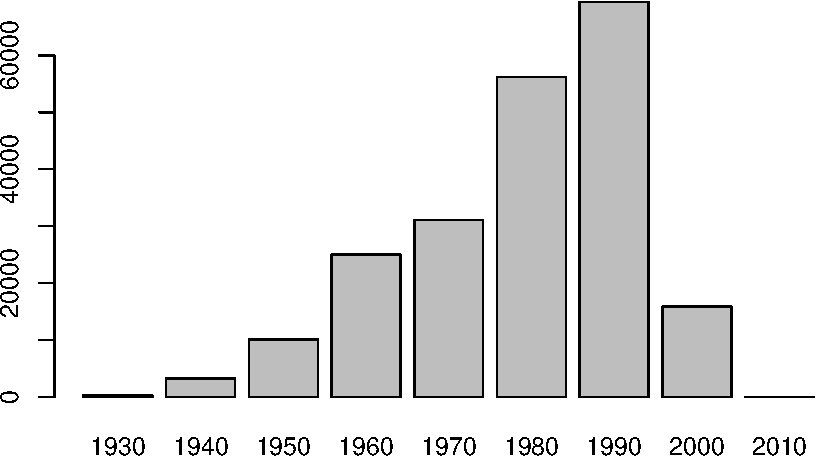
\includegraphics{R-data-wrangling_files/figure-latex/driver-birth-cohorts-1.pdf}
\caption{\label{fig:driver-birth-cohorts}Driver Birth Cohorts}
\end{figure}

\begin{quote}
Challenge

Create a new data frame from the \texttt{trafficstops} data that meets
the following criteria: contains only the \texttt{violation\_raw} column
for female drivers of age 50 that were stopped on a Sunday. For this add
a new column to your data frame called \texttt{weekday\_of\_stop}
containing the number of the weekday when the stop occurred. Use the
\texttt{wday()} function from \texttt{lubridate} (Sunday = 1).

Think about how the commands should be ordered to produce this data
frame!
\end{quote}

\section{What is
split-apply-combine?}\label{what-is-split-apply-combine}

Many data analysis tasks can be approached using the
\emph{split-apply-combine} paradigm: split the data into groups, apply
some analysis to each group, and then combine the results.

\begin{figure}
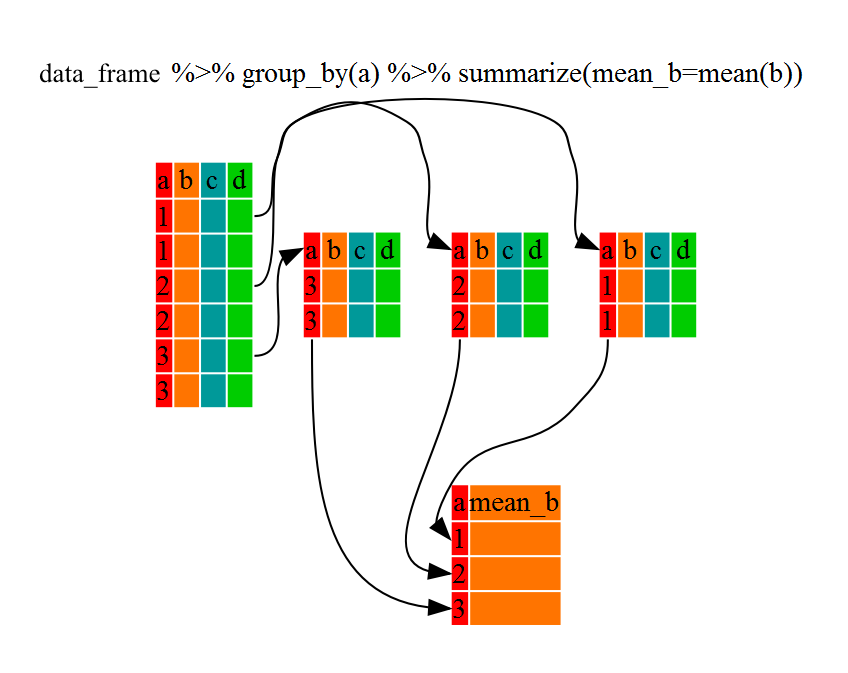
\includegraphics[width=\textwidth]{img/split-apply-combine} \caption{Split - Apply - Combine}\label{fig:split-apply-combine}
\end{figure}

\textbf{\texttt{dplyr}} makes this very easy through the use of the
\texttt{group\_by()} function.

\texttt{group\_by()} is often used together with \texttt{summarize()},
which collapses each group into a single-row summary of that group.
\texttt{group\_by()} takes as arguments the column names that contain
the \textbf{categorical} variables for which you want to calculate the
summary statistics. So to view the mean age for black and white drivers:

\begin{Shaded}
\begin{Highlighting}[]
\NormalTok{trafficstops }\OperatorTok
\StringTok{  }\KeywordTok{group_by}\NormalTok{(driver_race) }\OperatorTok
\StringTok{  }\KeywordTok{summarize}\NormalTok{(}\DataTypeTok{mean_age =} \KeywordTok{mean}\NormalTok{(driver_age, }\DataTypeTok{na.rm=}\OtherTok{TRUE}\NormalTok{))}
\end{Highlighting}
\end{Shaded}

\begin{verbatim}
#> # A tibble: 3 x 2
#>   driver_race mean_age
#>   <fct>          <dbl>
#> 1 Black           34.2
#> 2 White           36.2
#> 3 <NA>            34.5
\end{verbatim}

If we wanted to remove the line with \texttt{NA} we could insert a
\texttt{filter()} in the chain:

\begin{Shaded}
\begin{Highlighting}[]
\NormalTok{trafficstops }\OperatorTok
\StringTok{  }\KeywordTok{filter}\NormalTok{(}\OperatorTok{!}\KeywordTok{is.na}\NormalTok{(driver_race)) }\OperatorTok\StringTok{ }
\StringTok{  }\KeywordTok{group_by}\NormalTok{(driver_race) }\OperatorTok
\StringTok{  }\KeywordTok{summarize}\NormalTok{(}\DataTypeTok{mean_age =} \KeywordTok{mean}\NormalTok{(driver_age, }\DataTypeTok{na.rm=}\OtherTok{TRUE}\NormalTok{))}
\end{Highlighting}
\end{Shaded}

\begin{verbatim}
#> # A tibble: 2 x 2
#>   driver_race mean_age
#>   <fct>          <dbl>
#> 1 Black           34.2
#> 2 White           36.2
\end{verbatim}

Recall that \texttt{is.na()} is a function that determines whether
something is an \texttt{NA}. The \texttt{!} symbol negates the result,
so we're asking for everything that is \emph{not} an \texttt{NA}.

You may have noticed that the output from these calls looks a little
different. That's because \textbf{\texttt{dplyr}} has changed our
\texttt{data.frame} object to an object of class \texttt{tbl\_df}, also
known as a ``tibble''. Tibble's data structure is very similar to a data
frame. For our purposes the only differences are that (1) columns of
class \texttt{character} are never converted into factors, and (2) in
addition to displaying the data type of each column under its name, it
only prints the first few rows of data and only as many columns as fit
on one screen. If we wanted to print all columns we can use the print
command, and set the \texttt{width} parameter to \texttt{Inf}. To print
the first 6 rows for example we would do this:
\texttt{print(my\_tibble,\ n=6,\ width=Inf)}.

You can also group by multiple columns:

\begin{Shaded}
\begin{Highlighting}[]
\NormalTok{trafficstops }\OperatorTok\StringTok{ }
\StringTok{  }\KeywordTok{filter}\NormalTok{(}\OperatorTok{!}\KeywordTok{is.na}\NormalTok{(driver_race)) }\OperatorTok\StringTok{ }
\StringTok{  }\KeywordTok{group_by}\NormalTok{(driver_race, driver_gender) }\OperatorTok
\StringTok{  }\KeywordTok{summarize}\NormalTok{(}\DataTypeTok{mean_age =} \KeywordTok{mean}\NormalTok{(driver_age, }\DataTypeTok{na.rm=}\OtherTok{TRUE}\NormalTok{))}
\end{Highlighting}
\end{Shaded}

\begin{verbatim}
#> # A tibble: 4 x 3
#> # Groups:   driver_race [?]
#>   driver_race driver_gender mean_age
#>   <fct>       <fct>            <dbl>
#> 1 Black       female            33.1
#> 2 Black       male              35.2
#> 3 White       female            35.7
#> 4 White       male              36.5
\end{verbatim}

Once the data are grouped, you can also summarize multiple variables at
the same time (and not necessarily on the same variable). For instance,
we could add a column indicating the minimum age:

\begin{Shaded}
\begin{Highlighting}[]
\NormalTok{trafficstops }\OperatorTok\StringTok{ }
\StringTok{  }\KeywordTok{filter}\NormalTok{(}\OperatorTok{!}\KeywordTok{is.na}\NormalTok{(driver_race)) }\OperatorTok\StringTok{ }
\StringTok{  }\KeywordTok{group_by}\NormalTok{(driver_race, driver_gender) }\OperatorTok
\StringTok{  }\KeywordTok{summarize}\NormalTok{(}\DataTypeTok{mean_age =} \KeywordTok{mean}\NormalTok{(driver_age, }\DataTypeTok{na.rm=}\OtherTok{TRUE}\NormalTok{),}
            \DataTypeTok{min_age =} \KeywordTok{min}\NormalTok{(driver_age, }\DataTypeTok{na.rm=}\OtherTok{TRUE}\NormalTok{))}
\end{Highlighting}
\end{Shaded}

\begin{verbatim}
#> # A tibble: 4 x 4
#> # Groups:   driver_race [?]
#>   driver_race driver_gender mean_age min_age
#>   <fct>       <fct>            <dbl>   <dbl>
#> 1 Black       female            33.1      16
#> 2 Black       male              35.2       7
#> 3 White       female            35.7      15
#> 4 White       male              36.5      15
\end{verbatim}

\section{Tallying}\label{tallying}

When working with data, it is also common to want to know the number of
observations found for each factor or combination of factors. For this,
\textbf{\texttt{dplyr}} provides \texttt{tally()}. For example, if we
wanted to see how many traffic stops each officer recorded we would do:

\begin{Shaded}
\begin{Highlighting}[]
\NormalTok{trafficstops }\OperatorTok
\StringTok{  }\KeywordTok{group_by}\NormalTok{(officer_id) }\OperatorTok
\StringTok{  }\KeywordTok{tally}\NormalTok{()}
\end{Highlighting}
\end{Shaded}

Here, \texttt{tally()} is the action applied to the groups created by
\texttt{group\_by()} and counts the total number of records for each
category.

Alternatives:

\begin{Shaded}
\begin{Highlighting}[]
\NormalTok{trafficstops }\OperatorTok
\StringTok{  }\KeywordTok{count}\NormalTok{(officer_id) }\CommentTok{# count() calls group_by automatically, then tallies}

\NormalTok{trafficstops }\OperatorTok
\StringTok{  }\KeywordTok{group_by}\NormalTok{(officer_id) }\OperatorTok
\StringTok{  }\KeywordTok{summarize}\NormalTok{(}\DataTypeTok{n =} \KeywordTok{n}\NormalTok{()) }\CommentTok{# n() is useful when count is needed for a calculation}
\end{Highlighting}
\end{Shaded}

We can optionally sort the results in descending order by adding
\texttt{sort=TRUE}:

\begin{Shaded}
\begin{Highlighting}[]
\NormalTok{trafficstops }\OperatorTok
\StringTok{  }\KeywordTok{group_by}\NormalTok{(officer_id) }\OperatorTok
\StringTok{  }\KeywordTok{tally}\NormalTok{(}\DataTypeTok{sort=}\OtherTok{TRUE}\NormalTok{)}
\end{Highlighting}
\end{Shaded}

\begin{quote}
Challenge

Which 5 counties were the ones with the most stops in 2013? Hint: use
the year() function from lubridate.
\end{quote}

\section{Joining two tables}\label{joining-two-tables}

It is not uncommon that we have our data spread out in different tables
and need to bring those together for analysis. For example, to calculate
the proportion of stopped black and white drivers in relation to the
entire populations of white and black persons in each county we
introduce another table with that demographic information. These are the
estimated values of the 5 year average of the 2011-2015 American
Community Survey (ACS):

\begin{Shaded}
\begin{Highlighting}[]
\NormalTok{MS_bw_pop <-}\StringTok{ }\KeywordTok{read.csv}\NormalTok{(}\StringTok{"data/MS_acs2015_bw.csv"}\NormalTok{)}
\KeywordTok{head}\NormalTok{(MS_bw_pop)}
\end{Highlighting}
\end{Shaded}

\begin{verbatim}
#>    FIPS black_pop white_pop
#> 1 28001     17757     12856
#> 2 28003      4281     31563
#> 3 28005      5416      7395
#> 4 28007      8194     10649
#> 5 28009      3078      5166
#> 6 28011     21648     11197
\end{verbatim}

As unique ID, which uniquely identifies the corresponding records in
each table we use the
\href{https://en.wikipedia.org/wiki/Federal_Information_Processing_Standards}{FIPS
code}. It is stored in the \texttt{county\_fips} column in the
\texttt{trafficstops} data frame and in the \texttt{FIPS} column in
\texttt{MS\_bw\_pop}). \texttt{dplyr} makes it very easy to bring the
two tables together. We will use \texttt{left\_join} to bring the two
tables together into one:

\begin{Shaded}
\begin{Highlighting}[]
\NormalTok{trafficstops }\OperatorTok
\StringTok{  }\KeywordTok{left_join}\NormalTok{(MS_bw_pop, }\DataTypeTok{by =} \KeywordTok{c}\NormalTok{(}\StringTok{"county_fips"}\NormalTok{ =}\StringTok{ "FIPS"}\NormalTok{)) }\OperatorTok\StringTok{ }
\StringTok{  }\KeywordTok{head}\NormalTok{()}
\end{Highlighting}
\end{Shaded}

\begin{verbatim}
#>              id state  stop_date       county_name county_fips
#> 1 MS-2013-00001    MS 2013-01-01      Jones County       28067
#> 2 MS-2013-00002    MS 2013-01-01 Lauderdale County       28075
#> 3 MS-2013-00003    MS 2013-01-01       Pike County       28113
#> 4 MS-2013-00004    MS 2013-01-01    Hancock County       28045
#> 5 MS-2013-00005    MS 2013-01-01     Holmes County       28051
#> 6 MS-2013-00006    MS 2013-01-01    Jackson County       28059
#>            police_department driver_gender driver_birthdate driver_race
#> 1 Mississippi Highway Patrol          male       1950-06-14       Black
#> 2 Mississippi Highway Patrol          male       1967-04-06       Black
#> 3 Mississippi Highway Patrol          male       1974-04-15       Black
#> 4 Mississippi Highway Patrol          male       1981-03-23       White
#> 5 Mississippi Highway Patrol          male       1992-08-03       White
#> 6 Mississippi Highway Patrol        female       1960-05-02       White
#>                                                 violation_raw officer_id
#> 1                     Seat belt not used properly as required       J042
#> 2                                            Careless driving       B026
#> 3 Speeding - Regulated or posted speed limit and actual speed       M009
#> 4 Speeding - Regulated or posted speed limit and actual speed       K035
#> 5 Speeding - Regulated or posted speed limit and actual speed       D028
#> 6 Speeding - Regulated or posted speed limit and actual speed       K023
#>   driver_age        violation black_pop white_pop
#> 1         63        Seat belt     19711     47154
#> 2         46 Careless driving     33893     43482
#> 3         39         Speeding     21028     18282
#> 4         32         Speeding      4172     39686
#> 5         20         Speeding     15498      3105
#> 6         53         Speeding     30704    101686
\end{verbatim}

\texttt{dplyr} join functions are generally equivalent \texttt{merge}
from the base command, but there are a few advantages:

\begin{itemize}
\tightlist
\item
  rows are kept in existing order
\item
  much faster
\item
  tells you what keys you're merging by (if you don't supply)
\item
  also work with database tables.
\end{itemize}

\url{https://groups.google.com/d/msg/manipulatr/OuAPC4VyfIc/Qnt8mDfq0WwJ}

See \texttt{?dplyr::join} for all the possible joins.

Now that we got a little bit of an odd table, lets see how we can
reshape it to make more sense of it.

\chapter{\texorpdfstring{Data Manipulation using
\textbf{\texttt{tidyr}}}{Data Manipulation using tidyr}}\label{tidyr}

\begin{quote}
Learning Objectives

\begin{itemize}
\tightlist
\item
  Understand the concept of a wide and a long table format and for which
  purpose those formats are useful.
\item
  Understand what key-value pairs are.
\item
  Reshape a data frame from long to wide format and back with the
  \texttt{spread} and \texttt{gather} commands from the
  \textbf{\texttt{tidyr}} package.
\item
  Export a data frame to a .csv file.
\end{itemize}
\end{quote}

\begin{center}\rule{0.5\linewidth}{\linethickness}\end{center}

\texttt{dplyr} pairs nicely with \textbf{\texttt{tidyr}} which enables
you to swiftly convert between different data formats for plotting and
analysis.

The package \textbf{\texttt{tidyr}} addresses the common problem of
wanting to reshape your data for plotting and use by different R
functions. Sometimes we want data sets where we have one row per
observation. Sometimes we want a data frame where each observation type
has its own column, and rows are instead more aggregated groups - like
surveys, where each column represents an answer. Moving back and forth
between these formats is nontrivial, and \textbf{\texttt{tidyr}} gives
you tools for this and more sophisticated data manipulation.

To learn more about \textbf{\texttt{tidyr}} after the workshop, you may
want to check out this
\href{https://github.com/rstudio/cheatsheets/raw/master/data-import.pdf}{cheatsheet
about \textbf{\texttt{tidyr}}}.

\section{About long and wide table
format}\label{about-long-and-wide-table-format}

The `long' format is where:

\begin{itemize}
\tightlist
\item
  each column is a variable
\item
  each row is an observation
\end{itemize}

In the `long' format, you usually have 1 column for the observed
variable and the other columns are ID variables.

For the `wide' format each row is often a site/subject/patient and you
have multiple observation variables containing the same type of data.
These can be either repeated observations over time, or observation of
multiple variables (or a mix of both). You may find data input may be
simpler or some other applications may prefer the `wide' format.
However, many of \texttt{R}`s functions have been designed assuming you
have 'long' format data. This tutorial will help you efficiently
transform your data regardless of original format.

\begin{figure}
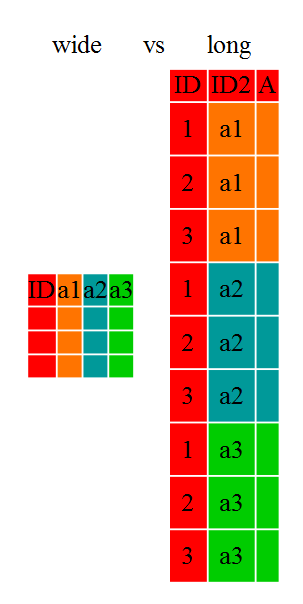
\includegraphics[width=0.3\linewidth]{img/wide-vs-long} \caption{Wide vs. Long Table Format}\label{fig:wide-vs-long}
\end{figure}

The choice of data format affects readability. For humans, the wide
format is often more intuitive, since we can often see more of the data
on the screen due to its shape. However, the long format is more machine
readable and is closer to the formatting of databases. The \texttt{ID}
variables in our dataframes are similar to the fields in a database and
observed variables are like the database values.

\begin{quote}
Challenge 1

Is trafficstops in a long or wide format?
\end{quote}

\section{\texorpdfstring{Long to Wide with
\texttt{spread}}{Long to Wide with spread}}\label{long-to-wide-with-spread}

Now let's see this in action. First, using \textbf{\texttt{dplyr}},
let's create a data frame with the mean age of each driver by gender and
county:

\begin{Shaded}
\begin{Highlighting}[]
\NormalTok{trafficstops_ma <-}\StringTok{ }\NormalTok{trafficstops }\OperatorTok
\StringTok{    }\KeywordTok{filter}\NormalTok{(}\OperatorTok{!}\KeywordTok{is.na}\NormalTok{(driver_gender)) }\OperatorTok
\StringTok{    }\KeywordTok{group_by}\NormalTok{(county_name, driver_gender) }\OperatorTok
\StringTok{    }\KeywordTok{summarize}\NormalTok{(}\DataTypeTok{mean_age =} \KeywordTok{mean}\NormalTok{(driver_age, }\DataTypeTok{na.rm =} \OtherTok{TRUE}\NormalTok{))}

\KeywordTok{head}\NormalTok{(trafficstops_ma)}
\end{Highlighting}
\end{Shaded}

\begin{verbatim}
#> # A tibble: 6 x 3
#> # Groups:   county_name [3]
#>   county_name   driver_gender mean_age
#>   <fct>         <fct>            <dbl>
#> 1 Adams County  female            36.7
#> 2 Adams County  male              38.4
#> 3 Alcorn County female            33.3
#> 4 Alcorn County male              34.1
#> 5 Amite County  female            38.3
#> 6 Amite County  male              40.3
\end{verbatim}

Now, to make this long data wide, we use \texttt{spread} from
\texttt{tidyr} to spread out the driver gender into columns.
\texttt{spread} takes three arguments - the data, the \emph{key} column,
or column with identifying information, the \emph{values} column - the
one with the numbers. We'll use a pipe so we can ignore the data
argument.

\begin{Shaded}
\begin{Highlighting}[]
\NormalTok{trafficstops_ma_wide <-}\StringTok{ }\NormalTok{trafficstops_ma }\OperatorTok
\StringTok{  }\KeywordTok{spread}\NormalTok{(driver_gender, mean_age) }

\KeywordTok{head}\NormalTok{(trafficstops_ma_wide)}
\end{Highlighting}
\end{Shaded}

\begin{verbatim}
#> # A tibble: 6 x 3
#> # Groups:   county_name [6]
#>   county_name    female  male
#>   <fct>           <dbl> <dbl>
#> 1 Adams County     36.7  38.4
#> 2 Alcorn County    33.3  34.1
#> 3 Amite County     38.3  40.3
#> 4 Attala County    36.7  38.1
#> 5 Benton County    32.1  34.4
#> 6 Bolivar County   33.2  36.3
\end{verbatim}

We can now do things like compare the mean age of men against women
drivers. As example we use the age difference to find the counties with
the largest and with the smallest number. (A negative number means that
female drivers are on average older than male drivers, a positive number
means that male drivers are on average older than women drivers.)

\begin{Shaded}
\begin{Highlighting}[]
\NormalTok{trafficstops_ma_wide }\OperatorTok\StringTok{ }
\StringTok{  }\KeywordTok{mutate}\NormalTok{(}\DataTypeTok{agediff =}\NormalTok{ male }\OperatorTok{-}\StringTok{ }\NormalTok{female) }\OperatorTok\StringTok{ }
\StringTok{  }\KeywordTok{ungroup}\NormalTok{() }\OperatorTok
\StringTok{  }\KeywordTok{filter}\NormalTok{(agediff }\OperatorTok\StringTok{ }\KeywordTok{range}\NormalTok{(agediff))}
\end{Highlighting}
\end{Shaded}

\begin{verbatim}
#> # A tibble: 2 x 4
#>   county_name      female  male agediff
#>   <fct>             <dbl> <dbl>   <dbl>
#> 1 Neshoba County     35.1  31.1   -3.94
#> 2 Yalobusha County   33.4  39.4    5.99
\end{verbatim}

Note that \texttt{trafficstops\_ma\_wide} is derived from
\texttt{trafficstops\_ma}, and is a ``grouped'' data frame, which was
created with the \texttt{group\_by} function above. (Check
\texttt{class(trafficstops\_ma)} and
\texttt{class(trafficstops\_ma\_wide)}). That means that any instruction
that follows will operate on each group (in this case county)
separately. That may be ok for some instances (like \texttt{mutate}),
but if we are interested in retreiveing the max and the min age
difference over all counties we need to \texttt{ungroup} the tibble to
have the \texttt{filter} command operate on the entire dataset.

\section{\texorpdfstring{Wide to long with
\texttt{gather}}{Wide to long with gather}}\label{wide-to-long-with-gather}

What if we had the opposite problem, and wanted to go from a wide to
long format? For that, we use \texttt{gather} to sweep up a set of
columns into one key-value pair. We give it the arguments of a new key
and value column name, and then we specify which columns we either want
or do not want gathered up. So, to go backwards from
\texttt{trafficstops\_ma\_wide}, and exclude \texttt{plot\_id} from the
gathering, we would do the following:

\begin{Shaded}
\begin{Highlighting}[]
\NormalTok{trafficstops_ma_long <-}\StringTok{ }\NormalTok{trafficstops_ma_wide }\OperatorTok
\StringTok{  }\KeywordTok{gather}\NormalTok{(gender, mean_age, }\OperatorTok{-}\NormalTok{county_name)}

\KeywordTok{head}\NormalTok{(trafficstops_ma_long)}
\end{Highlighting}
\end{Shaded}

\begin{verbatim}
#> # A tibble: 6 x 3
#> # Groups:   county_name [6]
#>   county_name    gender mean_age
#>   <fct>          <chr>     <dbl>
#> 1 Adams County   female     36.7
#> 2 Alcorn County  female     33.3
#> 3 Amite County   female     38.3
#> 4 Attala County  female     36.7
#> 5 Benton County  female     32.1
#> 6 Bolivar County female     33.2
\end{verbatim}

We could also have used a specification for what columns to include.
This can be useful if you have a large number of identifying columns,
and it's easier to specify what to gather than what to leave alone. And
if the columns are in a row, we don't even need to list them all out --
just use the \texttt{:} operator!

\begin{Shaded}
\begin{Highlighting}[]
\NormalTok{trafficstops_ma_wide }\OperatorTok
\StringTok{  }\KeywordTok{gather}\NormalTok{(gender, mean_age, female}\OperatorTok{:}\NormalTok{male) }\OperatorTok\StringTok{ }
\StringTok{  }\KeywordTok{head}\NormalTok{()}
\end{Highlighting}
\end{Shaded}

\begin{verbatim}
#> # A tibble: 6 x 3
#> # Groups:   county_name [6]
#>   county_name    gender mean_age
#>   <fct>          <chr>     <dbl>
#> 1 Adams County   female     36.7
#> 2 Alcorn County  female     33.3
#> 3 Amite County   female     38.3
#> 4 Attala County  female     36.7
#> 5 Benton County  female     32.1
#> 6 Bolivar County female     33.2
\end{verbatim}

\begin{quote}
Challenge

\begin{enumerate}
\def\labelenumi{\arabic{enumi}.}
\item
  Make a wide data frame with \texttt{year} as columns,
  \texttt{violation\_raw} as rows, and the values are the number of
  traffic stops per each violation. Use year() from the lubridate
  package. You will need to summarize before reshaping
\item
  Now take that data frame, and make it long again, so each row is a
  unique \texttt{violation\_raw} \texttt{year} combination.
\end{enumerate}
\end{quote}

Now that you have those commands under your belt, let's go back to our
table from before and reshape it so we can easily calculate the
percentage of black and white. To clean things up a little, we remove
rows where driver race is unknown.

We then make sure that we count our \texttt{NA}s as \texttt{0}. We know
from earlier that in Tunica County all reported stops are for black
drivers (Check again with:
\texttt{trafficstops\ \%\textgreater{}\%\ filter(county\_name\ ==\ "Tunica\ County")}).
By default spread would set the value for white stops to NA. Sometimes
it is fine to leave those as NA. Sometimes we want to fill them as
zeros, in which case we would add the argument \texttt{fill\ =\ 0}. In
our case we prefer to count this a 0.

Lastly, we introduce a separator (\texttt{sep}) as parameter to the
spread command. If \texttt{sep} is not \texttt{NULL}, the column names
will be given by
\texttt{"\textless{}key\_name\textgreater{}\textless{}sep\textgreater{}\textless{}key\_value\textgreater{}"}
and make them more explicit, easier for you to interpret, and for anyone
who might use your data.

\begin{Shaded}
\begin{Highlighting}[]
\NormalTok{trafficstops }\OperatorTok\StringTok{ }
\StringTok{  }\KeywordTok{filter}\NormalTok{(}\OperatorTok{!}\KeywordTok{is.na}\NormalTok{(driver_race)) }\OperatorTok\StringTok{ }
\StringTok{  }\KeywordTok{count}\NormalTok{(county_name, county_fips, driver_race) }\OperatorTok\StringTok{ }
\StringTok{  }\KeywordTok{spread}\NormalTok{(driver_race, n, }\DataTypeTok{fill =} \DecValTok{0}\NormalTok{, }\DataTypeTok{sep =} \StringTok{"_"}\NormalTok{) }\OperatorTok\StringTok{ }
\StringTok{  }\KeywordTok{head}\NormalTok{()}
\end{Highlighting}
\end{Shaded}

Now we can pipe this into our left join and calculate the percentages:

\begin{Shaded}
\begin{Highlighting}[]
\CommentTok{# make sure you this table loaded:}
\NormalTok{MS_bw_pop <-}\StringTok{ }\KeywordTok{read.csv}\NormalTok{(}\StringTok{"data/MS_acs2015_bw.csv"}\NormalTok{)}

\NormalTok{trafficstops }\OperatorTok\StringTok{ }
\StringTok{  }\KeywordTok{filter}\NormalTok{(}\OperatorTok{!}\KeywordTok{is.na}\NormalTok{(driver_race)) }\OperatorTok\StringTok{ }
\StringTok{  }\KeywordTok{count}\NormalTok{(county_name, county_fips, driver_race) }\OperatorTok\StringTok{ }
\StringTok{  }\KeywordTok{spread}\NormalTok{(driver_race, n, }\DataTypeTok{fill =} \DecValTok{0}\NormalTok{, }\DataTypeTok{sep =} \StringTok{"_"}\NormalTok{) }\OperatorTok\StringTok{  }
\StringTok{  }\KeywordTok{left_join}\NormalTok{(MS_bw_pop, }\DataTypeTok{by =} \KeywordTok{c}\NormalTok{(}\StringTok{"county_fips"}\NormalTok{ =}\StringTok{ "FIPS"}\NormalTok{)) }\OperatorTok\StringTok{ }
\StringTok{  }\KeywordTok{mutate}\NormalTok{(}\DataTypeTok{pct_black_stopped =}\NormalTok{ driver_race_Black}\OperatorTok{/}\NormalTok{black_pop,}
         \DataTypeTok{pct_white_stopped =}\NormalTok{ driver_race_White}\OperatorTok{/}\NormalTok{white_pop) }\OperatorTok\StringTok{ }
\StringTok{  }\KeywordTok{print}\NormalTok{(}\DataTypeTok{n=}\DecValTok{5}\NormalTok{, }\DataTypeTok{width=}\OtherTok{Inf}\NormalTok{)}
\end{Highlighting}
\end{Shaded}

\begin{verbatim}
#> # A tibble: 82 x 8
#>   county_name   county_fips driver_race_Black driver_race_White black_pop
#>   <fct>               <int>             <dbl>             <dbl>     <int>
#> 1 Adams County        28001               583               359     17757
#> 2 Alcorn County       28003               468              2877      4281
#> 3 Amite County        28005              1589              1331      5416
#> 4 Attala County       28007              2096              2107      8194
#> 5 Benton County       28009               121                93      3078
#>   white_pop pct_black_stopped pct_white_stopped
#>       <int>             <dbl>             <dbl>
#> 1     12856            0.0328            0.0279
#> 2     31563            0.109             0.0912
#> 3      7395            0.293             0.180 
#> 4     10649            0.256             0.198 
#> 5      5166            0.0393            0.0180
#> # ... with 77 more rows
\end{verbatim}

Terrific.

Now let's use some visualization to help us understand our data. Before
we do this though, let's save this table out.

\section{Exporting data}\label{exporting-data}

Instead of printing the above output to the screen we will pipe it into
another command. Similar to the \texttt{read.csv()} function used for
reading CSV files into R, there is a \texttt{write.csv()} function that
generates CSV files from data frames.

Before using \texttt{write.csv()}, we are going to create a new folder,
\texttt{data\_output}, in our working directory that will store this
generated dataset. We don't want to write generated datasets in the same
directory as our raw data. It's good practice to keep them separate. The
\texttt{data} folder should only contain the raw, unaltered data, and
should be left alone to make sure we don't delete or modify it. In
contrast, our script will generate the contents of the
\texttt{data\_output} directory, so even if the files it contains are
deleted, we can always re-generate them.

We can save the table generated by the join as a CSV file in our
\texttt{data\_output} folder. By default, \texttt{write.csv()} includes
a column with row names (in our case the names are just the row
numbers), so we need to add \texttt{row.names\ =\ FALSE} so they are not
included:

\begin{Shaded}
\begin{Highlighting}[]
\NormalTok{trafficstops }\OperatorTok\StringTok{ }
\StringTok{  }\KeywordTok{filter}\NormalTok{(}\OperatorTok{!}\KeywordTok{is.na}\NormalTok{(driver_race)) }\OperatorTok\StringTok{ }
\StringTok{  }\KeywordTok{count}\NormalTok{(county_name, county_fips, driver_race) }\OperatorTok\StringTok{ }
\StringTok{  }\KeywordTok{spread}\NormalTok{(driver_race, n, }\DataTypeTok{fill =} \DecValTok{0}\NormalTok{, }\DataTypeTok{sep =} \StringTok{"_"}\NormalTok{) }\OperatorTok\StringTok{  }
\StringTok{  }\KeywordTok{left_join}\NormalTok{(MS_bw_pop, }\DataTypeTok{by =} \KeywordTok{c}\NormalTok{(}\StringTok{"county_fips"}\NormalTok{ =}\StringTok{ "FIPS"}\NormalTok{)) }\OperatorTok\StringTok{ }
\StringTok{  }\KeywordTok{mutate}\NormalTok{(}\DataTypeTok{pct_black_stopped =}\NormalTok{ driver_race_Black}\OperatorTok{/}\NormalTok{black_pop,}
         \DataTypeTok{pct_white_stopped =}\NormalTok{ driver_race_White}\OperatorTok{/}\NormalTok{white_pop) }\OperatorTok\StringTok{ }
\StringTok{  }\KeywordTok{write.csv}\NormalTok{(}\DataTypeTok{file =} \StringTok{"data_output/MS_demographic.csv"}\NormalTok{, }\DataTypeTok{row.names =} \OtherTok{FALSE}\NormalTok{)}
\end{Highlighting}
\end{Shaded}

\chapter{\texorpdfstring{Data Visualization with
\texttt{ggplot2}}{Data Visualization with ggplot2}}\label{data-visualization-with-ggplot2}

\begin{quote}
Learning Objectives

\begin{itemize}
\tightlist
\item
  Bind a data frame to a plot
\item
  Select variables to be plotted and variables to define the
  presentation such as size, shape, color, transparency, etc. by
  defining aesthetics (\texttt{aes})
\item
  Add a graphical representation of the data in the plot (points, lines,
  bars) adding ``geoms'' layers
\item
  Produce scatter plots, barplots, boxplots, and line plots using
  ggplot.
\item
  Modify the aesthetics for the entire plot as well as for individual
  ``geoms'' layers
\item
  Modify plot elements (labels, text, scale, orientation)
\item
  Group observations by a factor variable
\item
  Break up plot into multiple panels (facetting)
\item
  Apply ggplot themes and create and apply customized themes
\item
  Save a plot created by ggplot as an image
\end{itemize}
\end{quote}

\begin{center}\rule{0.5\linewidth}{\linethickness}\end{center}

We start by loading the required packages. \textbf{\texttt{ggplot2}} is
included in the \textbf{\texttt{tidyverse}} package.

\begin{Shaded}
\begin{Highlighting}[]
\KeywordTok{library}\NormalTok{(tidyverse)}
\end{Highlighting}
\end{Shaded}

If not still in the workspace, load the data we saved in the previous
lesson.

\begin{Shaded}
\begin{Highlighting}[]
\NormalTok{MS_demographic <-}\StringTok{ }\KeywordTok{read.csv}\NormalTok{(}\StringTok{'data_output/MS_demographic.csv'}\NormalTok{)}
\end{Highlighting}
\end{Shaded}

(If you need to, you can also download the data from here:
\url{https://github.com/cengel/R-data-wrangling/raw/master/data_output/MS_demographic.csv})

\section{\texorpdfstring{Plotting with
\textbf{\texttt{ggplot2}}}{Plotting with ggplot2}}\label{plotting-with-ggplot2}

\textbf{\texttt{ggplot2}} is a plotting package that makes it simple to
create complex plots from data in a data frame. It provides a more
programmatic interface for specifying what variables to plot, how they
are displayed, and general visual properties, so we only need minimal
changes if the underlying data change or if we decide to change from a
bar plot to a scatterplot. This helps in creating publication quality
plots with minimal amounts of adjustments and tweaking.

ggplot generally likes data in the `long' format: i.e., a column for
every dimension, and a row for every observation. Well structured data
will save you lots of time when making figures with ggplot.

ggplot graphics are built step by step by adding new elements using the
\texttt{+} sign.

To build a ggplot we need to:

\begin{itemize}
\tightlist
\item
  bind the plot to a specific data frame using the \texttt{data}
  argument
\end{itemize}

\begin{Shaded}
\begin{Highlighting}[]
\KeywordTok{ggplot}\NormalTok{(}\DataTypeTok{data =}\NormalTok{ MS_demographic)}
\end{Highlighting}
\end{Shaded}

\begin{itemize}
\tightlist
\item
  define aesthetics (\texttt{aes}), by selecting the variables to be
  plotted and the variables to define the presentation such as plotting
  size, shape color, etc.
\end{itemize}

\begin{Shaded}
\begin{Highlighting}[]
\KeywordTok{ggplot}\NormalTok{(}\DataTypeTok{data =}\NormalTok{ MS_demographic, }\KeywordTok{aes}\NormalTok{(}\DataTypeTok{x =}\NormalTok{ pct_black_stopped, }\DataTypeTok{y =}\NormalTok{ pct_white_stopped))}
\end{Highlighting}
\end{Shaded}

\begin{itemize}
\tightlist
\item
  add ``geoms'' -- a graphical representation of the data in the plot
  (points, lines, bars). To add a geom to the plot use \texttt{+}
  operator
\end{itemize}

\begin{Shaded}
\begin{Highlighting}[]
\KeywordTok{ggplot}\NormalTok{(}\DataTypeTok{data =}\NormalTok{ MS_demographic, }\KeywordTok{aes}\NormalTok{(}\DataTypeTok{x =}\NormalTok{ pct_black_stopped, }\DataTypeTok{y =}\NormalTok{ pct_white_stopped)) }\OperatorTok{+}
\StringTok{  }\KeywordTok{geom_point}\NormalTok{()}
\end{Highlighting}
\end{Shaded}

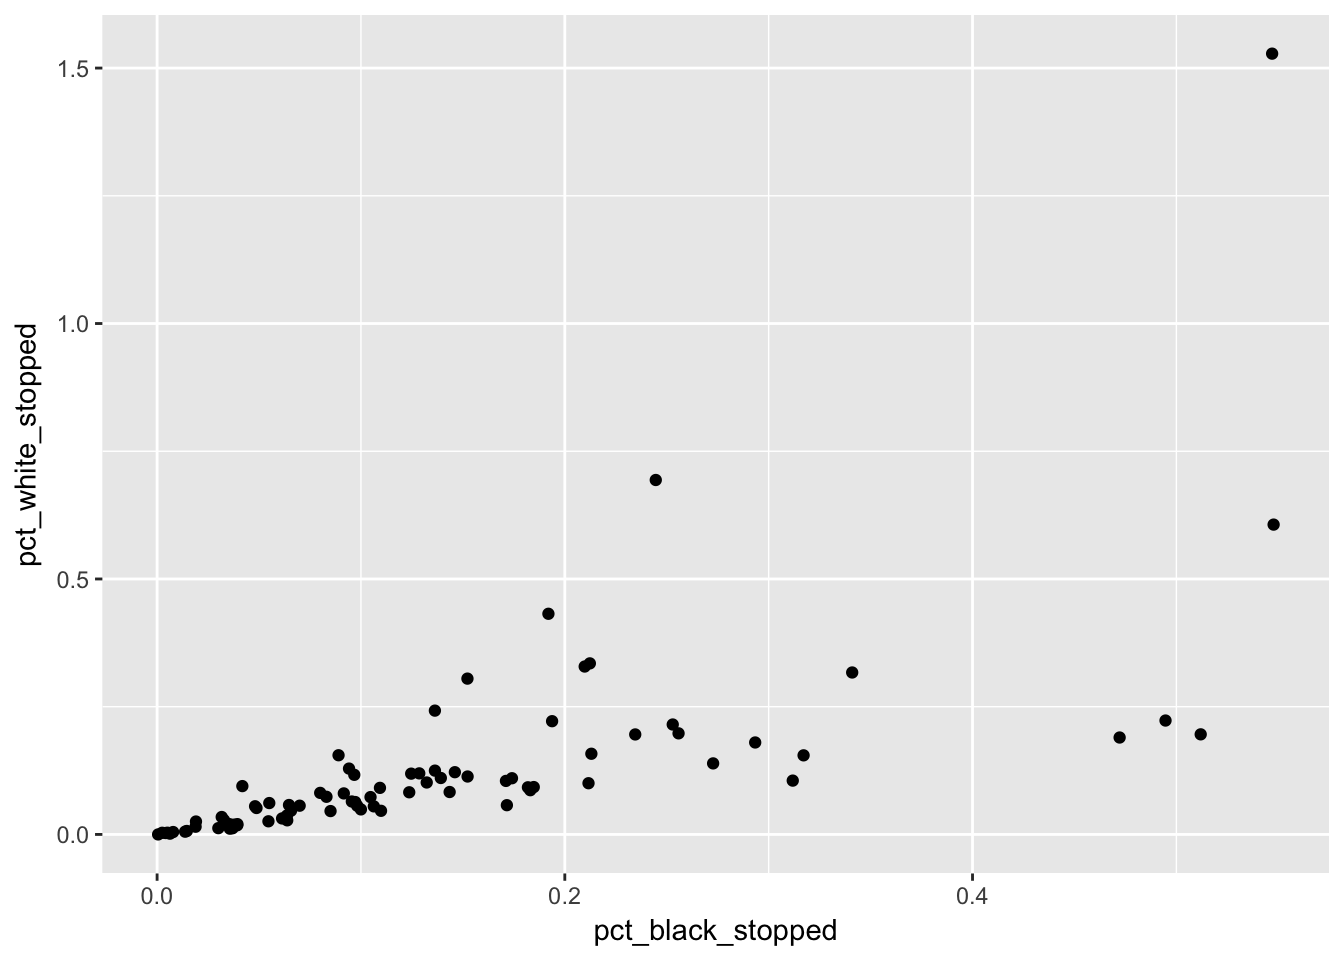
\includegraphics[width=0.7\linewidth]{R-data-wrangling_files/figure-latex/first-ggplot-1}

The \texttt{+} in the \textbf{\texttt{ggplot2}} package is particularly
useful because it allows you to modify existing \texttt{ggplot} objects.
This means you can easily set up plot ``templates'' and conveniently
explore different types of plots, so the above plot can also be
generated with code like this:

\begin{Shaded}
\begin{Highlighting}[]
\CommentTok{# Assign plot to a variable}
\NormalTok{MS_plot <-}\StringTok{ }\KeywordTok{ggplot}\NormalTok{(}\DataTypeTok{data =}\NormalTok{ MS_demographic, }\KeywordTok{aes}\NormalTok{(}\DataTypeTok{x =}\NormalTok{ pct_black_stopped, }\DataTypeTok{y =}\NormalTok{ pct_white_stopped))}

\CommentTok{# Draw the plot}
\NormalTok{MS_plot }\OperatorTok{+}\StringTok{ }\KeywordTok{geom_point}\NormalTok{()}
\end{Highlighting}
\end{Shaded}

Notes:

\begin{itemize}
\tightlist
\item
  Any parameters you set in the \texttt{ggplot()} function can be seen
  by any geom layers that you add (i.e., these are universal plot
  settings). This includes the x and y axis you set up in
  \texttt{aes()}.
\item
  Any parameters you set in the \texttt{geom\_*()} function are treated
  independently of (and override) the settings defined globally in the
  \texttt{ggplot()} function.
\item
  Geoms are plotted in the order they are added after each \texttt{+},
  that means geoms last added will display on top of prior geoms.
\item
  The \texttt{+} sign used to add layers \textbf{must be placed at the
  end of each line} containing a layer. If, instead, the \texttt{+} sign
  is added in the line before the other layer, \textbf{\texttt{ggplot2}}
  will not add the new layer and will return an error message.
\end{itemize}

\begin{Shaded}
\begin{Highlighting}[]
\CommentTok{# this is the correct syntax for adding layers}
\NormalTok{MS_plot }\OperatorTok{+}
\StringTok{  }\KeywordTok{geom_point}\NormalTok{()}

\CommentTok{# this will not add the new layer and will return an error message}
\NormalTok{MS_plot}
  \OperatorTok{+}\StringTok{ }\KeywordTok{geom_point}\NormalTok{()}
\end{Highlighting}
\end{Shaded}

To learn more about \textbf{\texttt{ggplot}} after the workshop, you may
want to check out this
\href{https://www.rstudio.com/wp-content/uploads/2016/11/ggplot2-cheatsheet-2.1.pdf}{cheatsheet
about \textbf{\texttt{ggplot}}}.

\section{Building your plots
iteratively}\label{building-your-plots-iteratively}

Building plots with ggplot can be of great help when you engage in
exploratory data analysis. It is typically an iterative process, where
you go back and forth between your data and their graphical
representation, which helps you in the process of getting to know your
data better.

Conveniently, \texttt{ggplot} works with pipes. The code below does the
same thing as above:

\begin{Shaded}
\begin{Highlighting}[]
\NormalTok{MS_demographic }\OperatorTok\StringTok{ }
\StringTok{  }\KeywordTok{ggplot}\NormalTok{(}\KeywordTok{aes}\NormalTok{(}\DataTypeTok{x =}\NormalTok{ pct_black_stopped, }\DataTypeTok{y =}\NormalTok{ pct_white_stopped)) }\OperatorTok{+}\StringTok{ }
\StringTok{  }\KeywordTok{geom_point}\NormalTok{() }
\end{Highlighting}
\end{Shaded}

We pipe the content of the table into \texttt{ggplot()}, so we can omit
the first (\texttt{data\ =} argument). Now let's use this to clean up a
few odd outliers in our data before we pass them to ggplot.

\begin{Shaded}
\begin{Highlighting}[]
\NormalTok{MS_demographic }\OperatorTok\StringTok{ }
\StringTok{  }\KeywordTok{filter}\NormalTok{(pct_white_stopped }\OperatorTok{<}\StringTok{ }\FloatTok{0.5} \OperatorTok{&}\StringTok{ }\NormalTok{pct_black_stopped }\OperatorTok{<}\StringTok{ }\FloatTok{0.5}\NormalTok{) }\OperatorTok\StringTok{ }
\StringTok{  }\KeywordTok{ggplot}\NormalTok{(}\KeywordTok{aes}\NormalTok{(}\DataTypeTok{x =}\NormalTok{ pct_black_stopped, }\DataTypeTok{y =}\NormalTok{ pct_white_stopped)) }\OperatorTok{+}\StringTok{ }
\StringTok{  }\KeywordTok{geom_point}\NormalTok{() }
\end{Highlighting}
\end{Shaded}

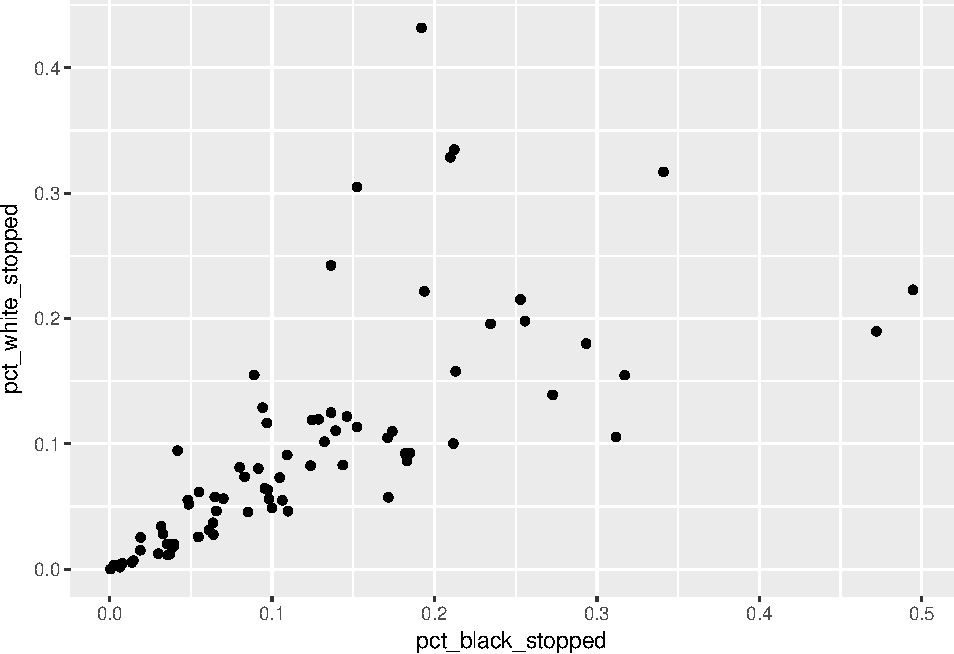
\includegraphics[width=0.7\linewidth]{R-data-wrangling_files/figure-latex/ggplot-with-filter-1}

Then we can start modifying this plot to extract more information from
it. For instance, we can add transparency (\texttt{alpha}) to avoid
overplotting:

\begin{Shaded}
\begin{Highlighting}[]
\NormalTok{MS_demographic }\OperatorTok\StringTok{ }
\StringTok{  }\KeywordTok{filter}\NormalTok{(pct_white_stopped }\OperatorTok{<}\StringTok{ }\FloatTok{0.5} \OperatorTok{&}\StringTok{ }\NormalTok{pct_black_stopped }\OperatorTok{<}\StringTok{ }\FloatTok{0.5}\NormalTok{) }\OperatorTok\StringTok{ }
\StringTok{  }\KeywordTok{ggplot}\NormalTok{(}\KeywordTok{aes}\NormalTok{(}\DataTypeTok{x =}\NormalTok{ pct_black_stopped, }\DataTypeTok{y =}\NormalTok{ pct_white_stopped)) }\OperatorTok{+}\StringTok{ }
\StringTok{  }\KeywordTok{geom_point}\NormalTok{(}\DataTypeTok{alpha =} \FloatTok{0.3}\NormalTok{)}
\end{Highlighting}
\end{Shaded}

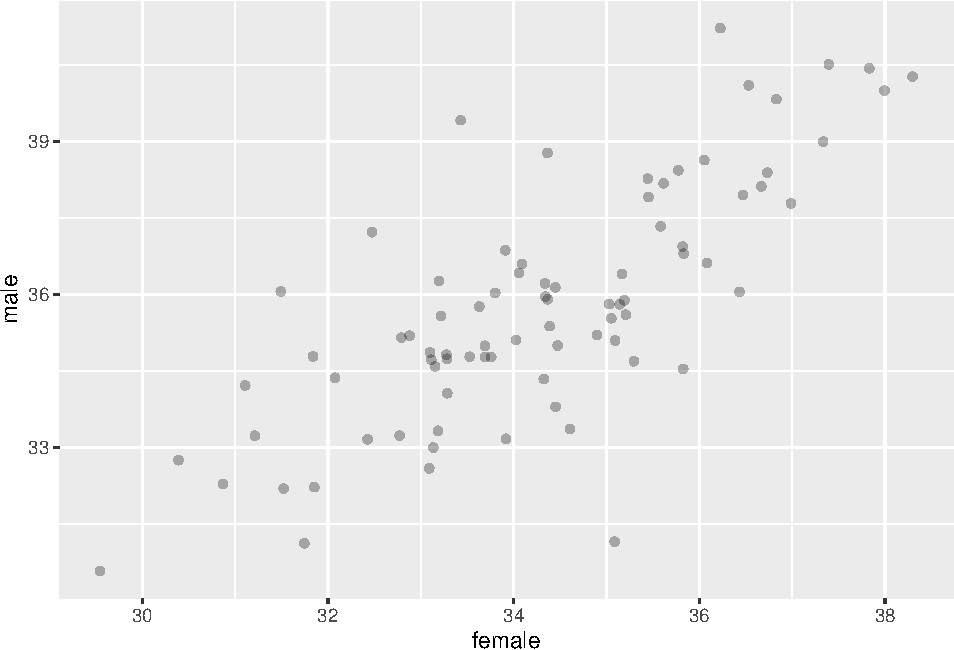
\includegraphics[width=0.7\linewidth]{R-data-wrangling_files/figure-latex/adding-transparency-1}

We can also add a color for all the points:

\begin{Shaded}
\begin{Highlighting}[]
\NormalTok{MS_demographic }\OperatorTok\StringTok{ }
\StringTok{  }\KeywordTok{filter}\NormalTok{(pct_white_stopped }\OperatorTok{<}\StringTok{ }\FloatTok{0.5} \OperatorTok{&}\StringTok{ }\NormalTok{pct_black_stopped }\OperatorTok{<}\StringTok{ }\FloatTok{0.5}\NormalTok{) }\OperatorTok\StringTok{ }
\StringTok{  }\KeywordTok{ggplot}\NormalTok{(}\KeywordTok{aes}\NormalTok{(}\DataTypeTok{x =}\NormalTok{ pct_black_stopped, }\DataTypeTok{y =}\NormalTok{ pct_white_stopped)) }\OperatorTok{+}\StringTok{ }
\StringTok{  }\KeywordTok{geom_point}\NormalTok{(}\DataTypeTok{alpha =} \FloatTok{0.3}\NormalTok{, }\DataTypeTok{color=} \StringTok{"blue"}\NormalTok{)}
\end{Highlighting}
\end{Shaded}

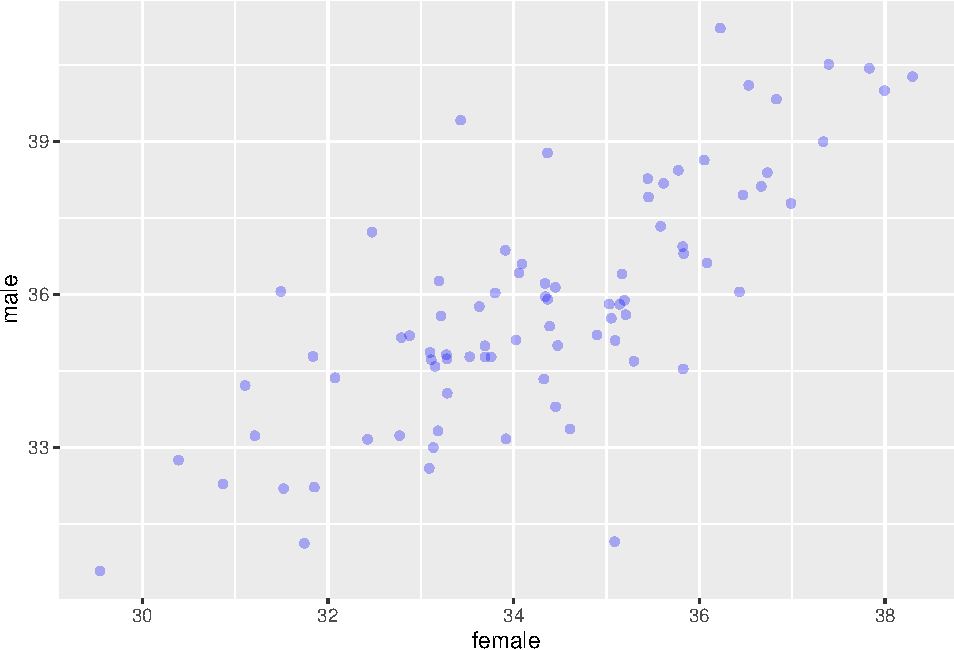
\includegraphics[width=0.7\linewidth]{R-data-wrangling_files/figure-latex/adding-color-1}

We can add another layer to the plot with \texttt{+}:

\begin{Shaded}
\begin{Highlighting}[]
\NormalTok{MS_demographic }\OperatorTok\StringTok{ }
\StringTok{  }\KeywordTok{filter}\NormalTok{(pct_white_stopped }\OperatorTok{<}\StringTok{ }\FloatTok{0.5} \OperatorTok{&}\StringTok{ }\NormalTok{pct_black_stopped }\OperatorTok{<}\StringTok{ }\FloatTok{0.5}\NormalTok{) }\OperatorTok\StringTok{ }
\StringTok{  }\KeywordTok{ggplot}\NormalTok{(}\KeywordTok{aes}\NormalTok{(}\DataTypeTok{x =}\NormalTok{ pct_black_stopped, }\DataTypeTok{y =}\NormalTok{ pct_white_stopped)) }\OperatorTok{+}\StringTok{ }
\StringTok{  }\KeywordTok{geom_point}\NormalTok{(}\DataTypeTok{alpha =} \FloatTok{0.3}\NormalTok{, }\DataTypeTok{color=} \StringTok{"blue"}\NormalTok{) }\OperatorTok{+}
\StringTok{  }\KeywordTok{geom_abline}\NormalTok{(}\DataTypeTok{intercept =} \DecValTok{0}\NormalTok{)}
\end{Highlighting}
\end{Shaded}

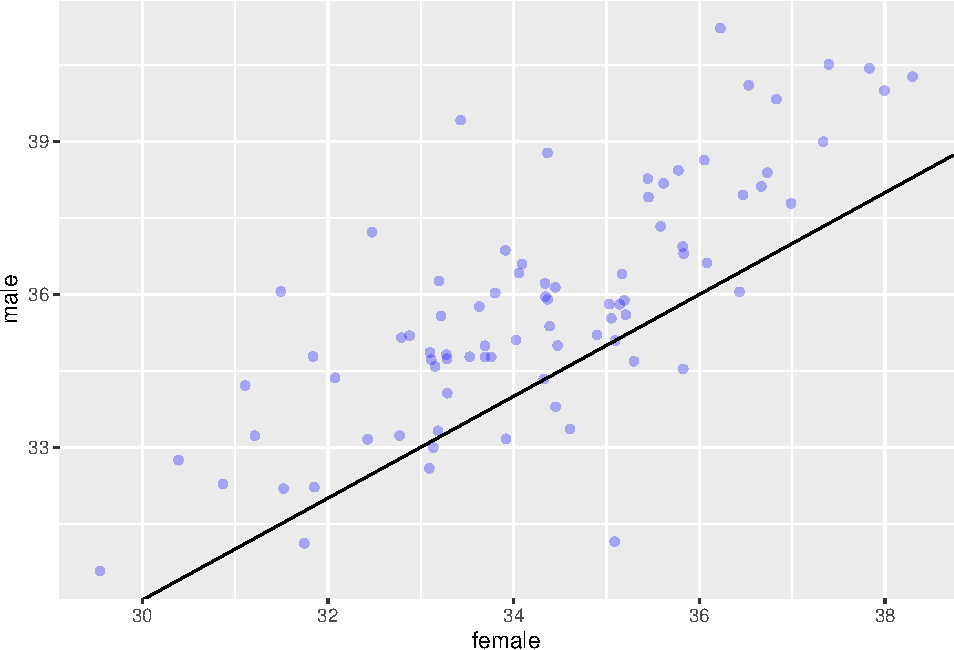
\includegraphics[width=0.7\linewidth]{R-data-wrangling_files/figure-latex/add-abline-1}

If we wanted to ``zoom'' into the plot, we could filter to a smaller
range of values before passing them to ggplot, but we can also tell
ggplot to only plot the x and y values for certain ranges. For this we
use \texttt{scale\_x\_continuous} and \texttt{scale\_y\_continuous}. You
will receive a message from ggplot telling you how many rows it has
removed from the plot.

\begin{Shaded}
\begin{Highlighting}[]
\NormalTok{MS_demographic }\OperatorTok\StringTok{ }
\StringTok{  }\KeywordTok{filter}\NormalTok{(pct_white_stopped }\OperatorTok{<}\StringTok{ }\FloatTok{0.5} \OperatorTok{&}\StringTok{ }\NormalTok{pct_black_stopped }\OperatorTok{<}\StringTok{ }\FloatTok{0.5}\NormalTok{) }\OperatorTok\StringTok{ }
\StringTok{  }\KeywordTok{ggplot}\NormalTok{(}\KeywordTok{aes}\NormalTok{(}\DataTypeTok{x =}\NormalTok{ pct_black_stopped, }\DataTypeTok{y =}\NormalTok{ pct_white_stopped)) }\OperatorTok{+}\StringTok{ }
\StringTok{  }\KeywordTok{geom_point}\NormalTok{(}\DataTypeTok{alpha =} \FloatTok{0.3}\NormalTok{, }\DataTypeTok{color=} \StringTok{"blue"}\NormalTok{) }\OperatorTok{+}
\StringTok{  }\KeywordTok{geom_abline}\NormalTok{(}\DataTypeTok{intercept =} \DecValTok{0}\NormalTok{) }\OperatorTok{+}\StringTok{ }
\StringTok{  }\KeywordTok{scale_x_continuous}\NormalTok{(}\DataTypeTok{limits =} \KeywordTok{c}\NormalTok{(}\DecValTok{0}\NormalTok{, }\FloatTok{0.1}\NormalTok{)) }\OperatorTok{+}
\StringTok{  }\KeywordTok{scale_y_continuous}\NormalTok{(}\DataTypeTok{limits =} \KeywordTok{c}\NormalTok{(}\DecValTok{0}\NormalTok{, }\FloatTok{0.1}\NormalTok{)) }
\end{Highlighting}
\end{Shaded}

\begin{verbatim}
#> Warning: Removed 40 rows containing missing values (geom_point).
\end{verbatim}

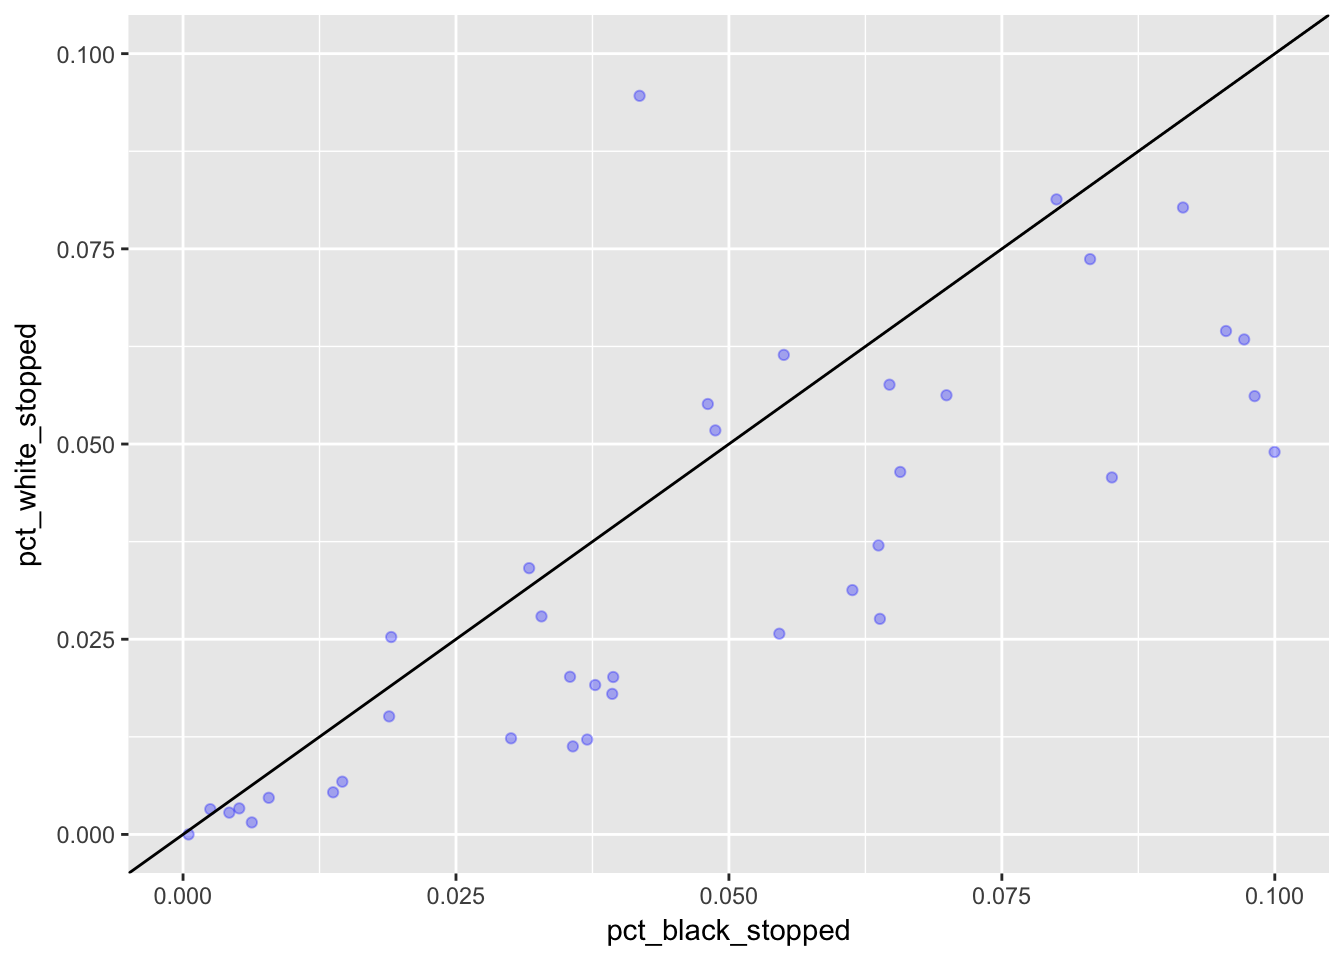
\includegraphics[width=0.7\linewidth]{R-data-wrangling_files/figure-latex/zoom-in-1}

\begin{quote}
Challenge

Modify the plot above to display different color for both points and
abline, and show a different range of data. How might you change the
size of the dots?
\end{quote}

\section{Barplot}\label{barplot}

There are two types of bar charts in ggplot, \texttt{geom\_bar} and
\texttt{geom\_col}. \texttt{geom\_bar} makes the height of the bar
proportional to the number of cases in each group and counts the number
of cases at each x position.

If we wanted to see how many violations we have of each type could say:

\begin{Shaded}
\begin{Highlighting}[]
\KeywordTok{ggplot}\NormalTok{(trafficstops, }\KeywordTok{aes}\NormalTok{(violation)) }\OperatorTok{+}\StringTok{ }
\StringTok{  }\KeywordTok{geom_bar}\NormalTok{()}
\end{Highlighting}
\end{Shaded}

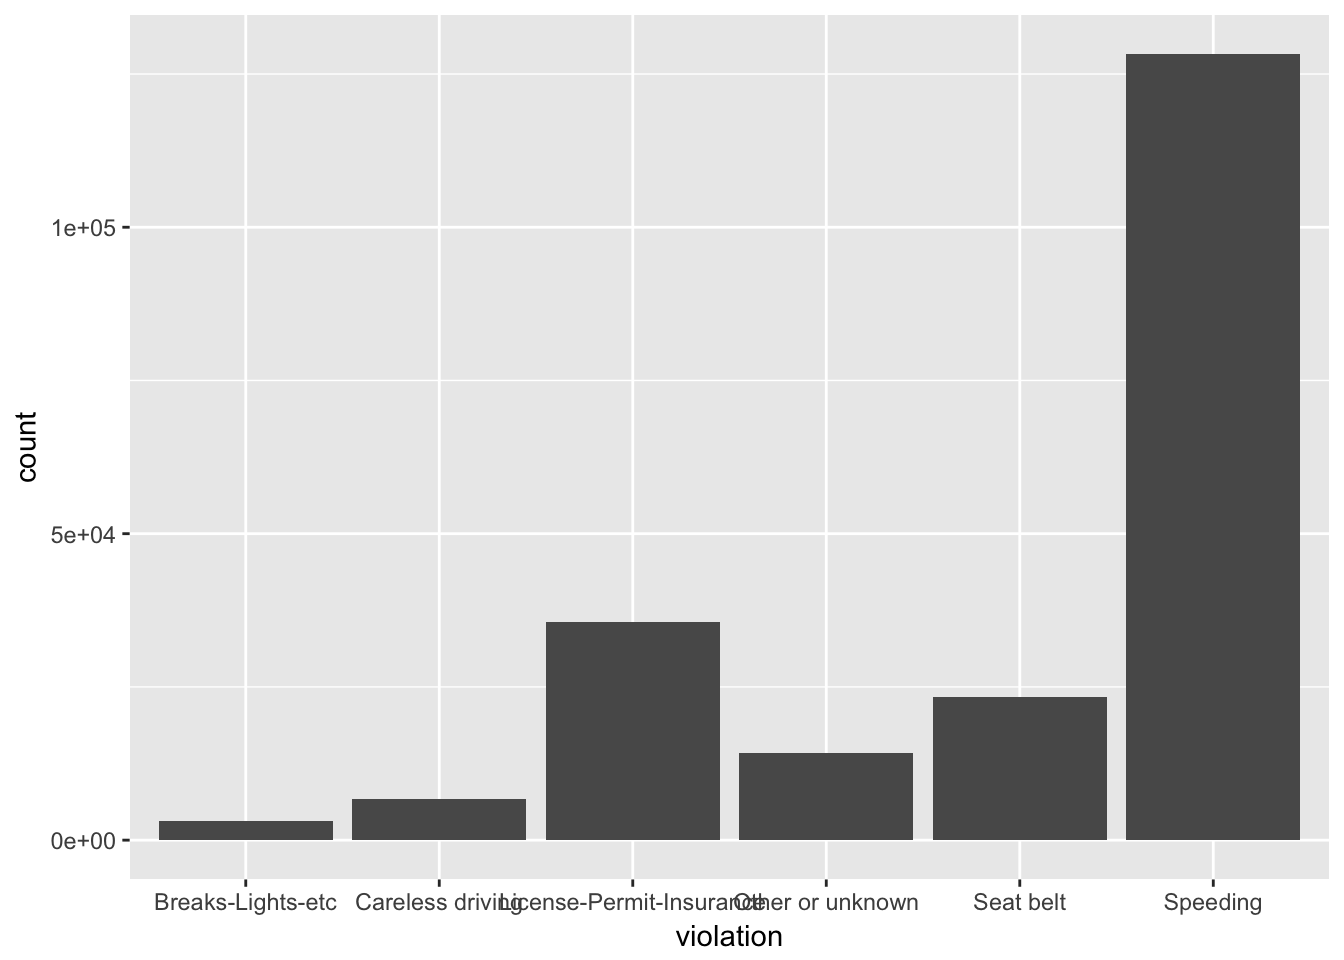
\includegraphics[width=0.7\linewidth]{R-data-wrangling_files/figure-latex/simple-bar-1}

As we have seen we could color the bars, but instead of \texttt{color}
we use \texttt{fill}. (What happens when you use \texttt{color}?)

\begin{Shaded}
\begin{Highlighting}[]
\KeywordTok{ggplot}\NormalTok{(trafficstops, }\KeywordTok{aes}\NormalTok{(violation)) }\OperatorTok{+}\StringTok{ }
\StringTok{  }\KeywordTok{geom_bar}\NormalTok{(}\DataTypeTok{fill =} \StringTok{"green"}\NormalTok{)}
\end{Highlighting}
\end{Shaded}

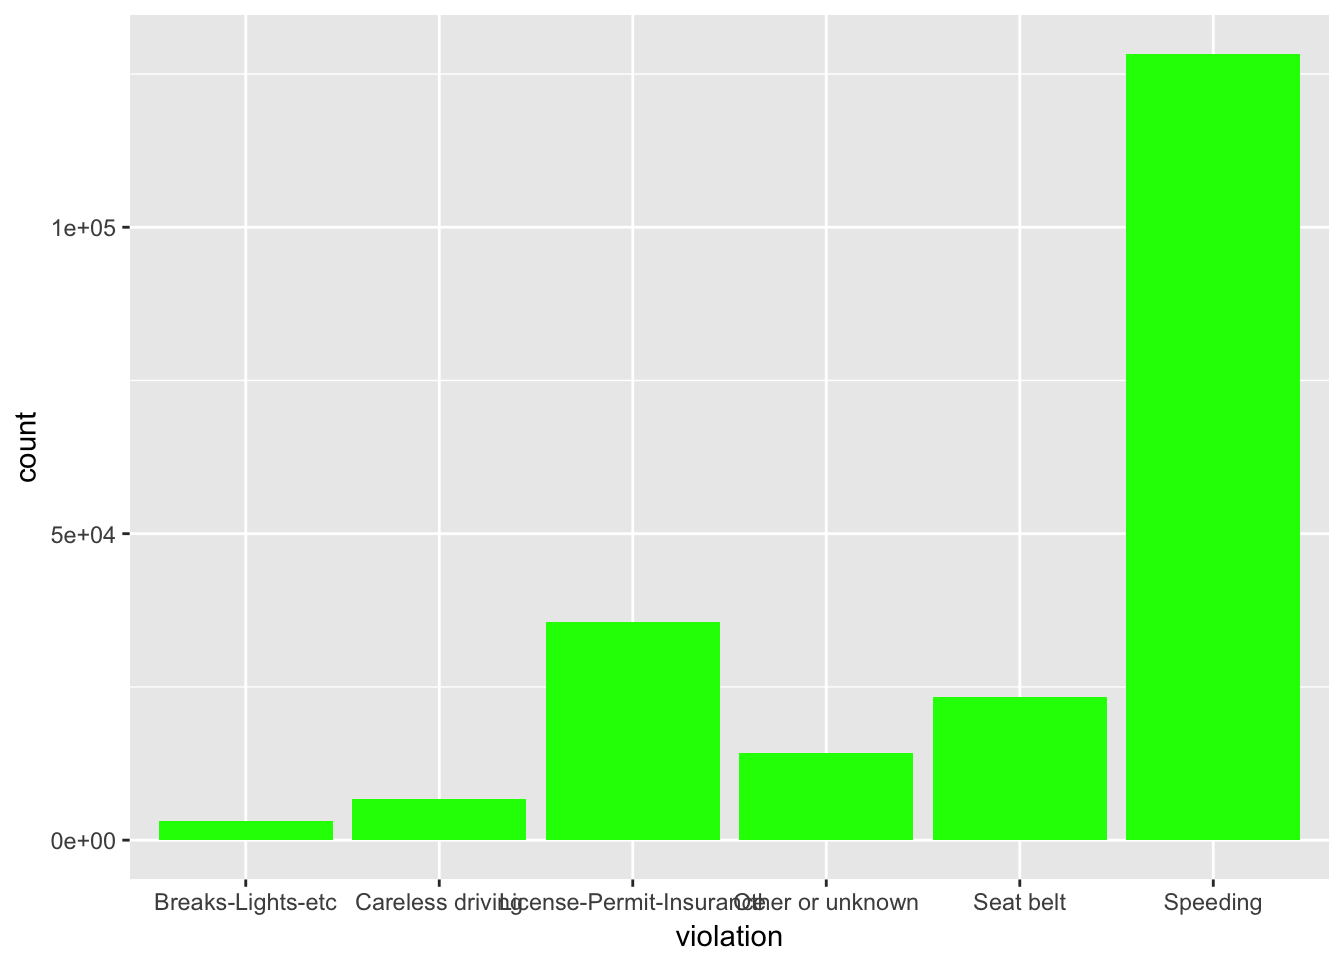
\includegraphics[width=0.7\linewidth]{R-data-wrangling_files/figure-latex/color-bar-simple-1}

Instead of coloring everything the same we could also color by another
category, say gender. For this we have to set the parameter within the
\texttt{aes()} function, which takes care of mapping the values to
different colors:

\begin{Shaded}
\begin{Highlighting}[]
\KeywordTok{ggplot}\NormalTok{(trafficstops, }\KeywordTok{aes}\NormalTok{(violation)) }\OperatorTok{+}\StringTok{ }
\StringTok{  }\KeywordTok{geom_bar}\NormalTok{(}\KeywordTok{aes}\NormalTok{(}\DataTypeTok{fill =}\NormalTok{ driver_gender))}
\end{Highlighting}
\end{Shaded}

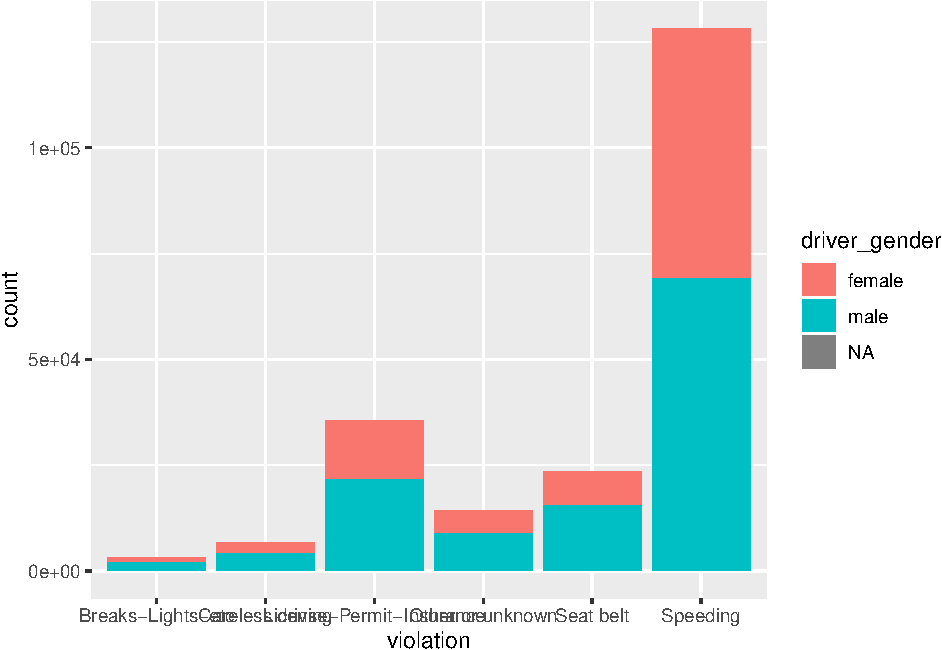
\includegraphics[width=0.7\linewidth]{R-data-wrangling_files/figure-latex/color-bar-gender-1}

If we wanted to see the proportions within each category we can tell
ggplot to stretch the bars between 0 and 1, we can set the position
parameter to `fill':

\begin{Shaded}
\begin{Highlighting}[]
\KeywordTok{ggplot}\NormalTok{(trafficstops, }\KeywordTok{aes}\NormalTok{(violation)) }\OperatorTok{+}\StringTok{ }
\StringTok{  }\KeywordTok{geom_bar}\NormalTok{(}\KeywordTok{aes}\NormalTok{(}\DataTypeTok{fill =}\NormalTok{ driver_gender), }\DataTypeTok{position =} \StringTok{"fill"}\NormalTok{)}
\end{Highlighting}
\end{Shaded}

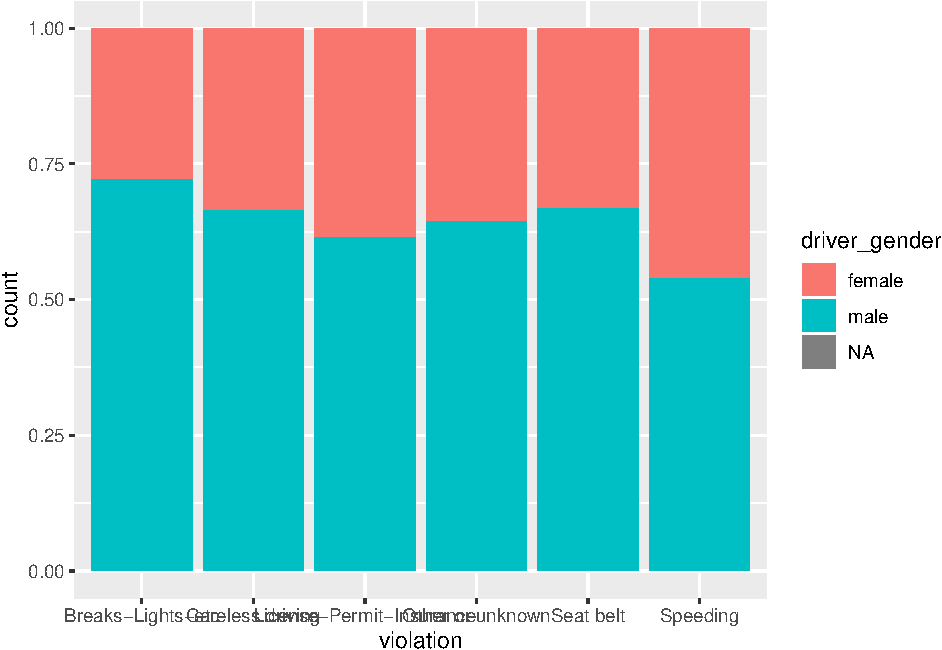
\includegraphics[width=0.7\linewidth]{R-data-wrangling_files/figure-latex/color-bar-stretch-1}

The other type of barchart, \texttt{geom\_col}, is used if you want the
heights of the bars to represent values in the data. It leaves the data
as is. For example, we can use \texttt{geom\_col} for a different way of
visualizing the data shown in the scatterplot above. For readability I
have also flipped the coordinates:

\begin{Shaded}
\begin{Highlighting}[]
\NormalTok{MS_demographic }\OperatorTok\StringTok{   }
\StringTok{  }\KeywordTok{filter}\NormalTok{(pct_white_stopped }\OperatorTok{<}\StringTok{ }\FloatTok{0.5} \OperatorTok{&}\StringTok{ }\NormalTok{pct_black_stopped }\OperatorTok{<}\StringTok{ }\FloatTok{0.5}\NormalTok{) }\OperatorTok
\StringTok{  }\KeywordTok{ggplot}\NormalTok{(}\KeywordTok{aes}\NormalTok{(}\DataTypeTok{x =}\NormalTok{ county_name, }\DataTypeTok{y =}\NormalTok{ pct_white_stopped }\OperatorTok{-}\StringTok{ }\NormalTok{pct_black_stopped)) }\OperatorTok{+}\StringTok{ }
\StringTok{    }\KeywordTok{geom_col}\NormalTok{() }\OperatorTok{+}\StringTok{ }
\StringTok{    }\KeywordTok{coord_flip}\NormalTok{()}
\end{Highlighting}
\end{Shaded}

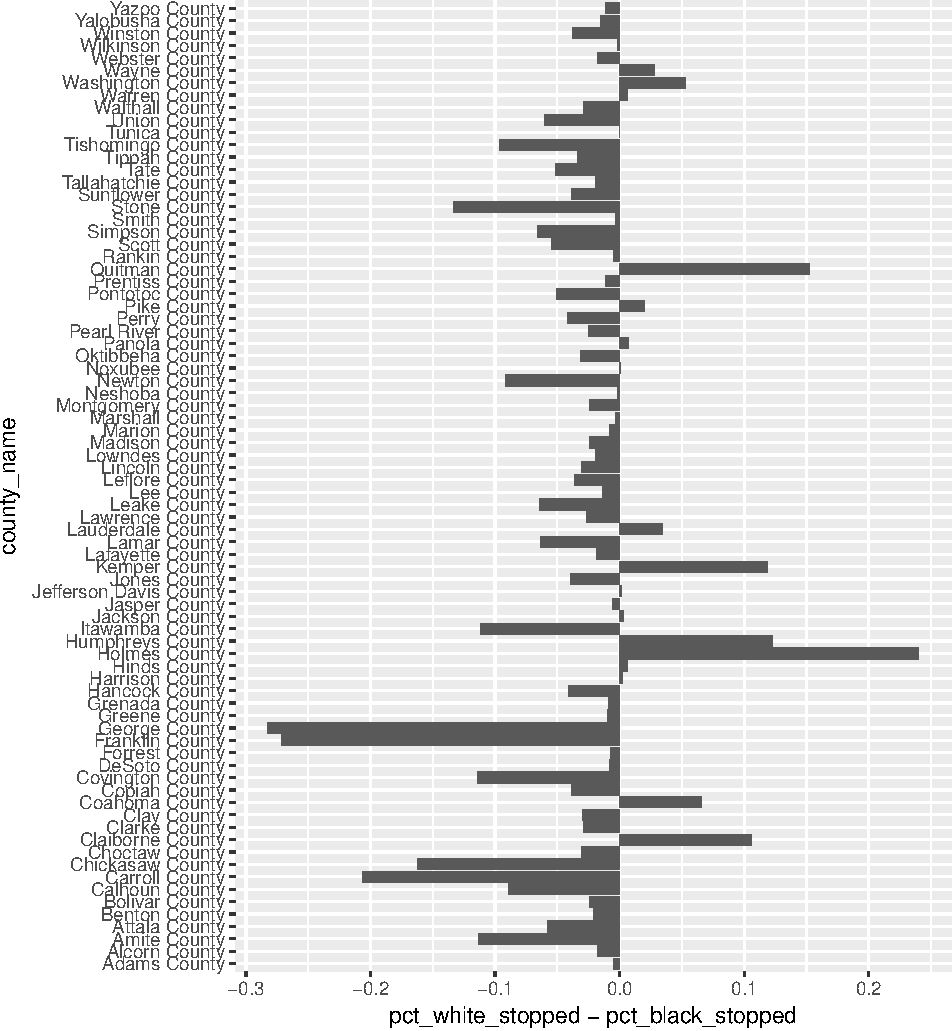
\includegraphics{R-data-wrangling_files/figure-latex/demograph-barplot-1.pdf}

\begin{quote}
Challenge

Make a barplot that shows for each race the proportion of stops for male
and female drivers. How could you get rid of the NAs?
\end{quote}

\section{Boxplot}\label{boxplot}

For this segment let's extract and work with the stops for Chickasaw
County only.

\begin{Shaded}
\begin{Highlighting}[]
\NormalTok{Chickasaw_stops <-}\StringTok{ }\KeywordTok{filter}\NormalTok{(trafficstops, county_name }\OperatorTok{==}\StringTok{ "Chickasaw County"}\NormalTok{)}
\end{Highlighting}
\end{Shaded}

We can use boxplots to visualize the distribution of driver age within
each violation:

\begin{Shaded}
\begin{Highlighting}[]
\KeywordTok{ggplot}\NormalTok{(}\DataTypeTok{data =}\NormalTok{ Chickasaw_stops, }\KeywordTok{aes}\NormalTok{(}\DataTypeTok{x =}\NormalTok{ violation, }\DataTypeTok{y =}\NormalTok{ driver_age)) }\OperatorTok{+}
\StringTok{    }\KeywordTok{geom_boxplot}\NormalTok{()}
\end{Highlighting}
\end{Shaded}

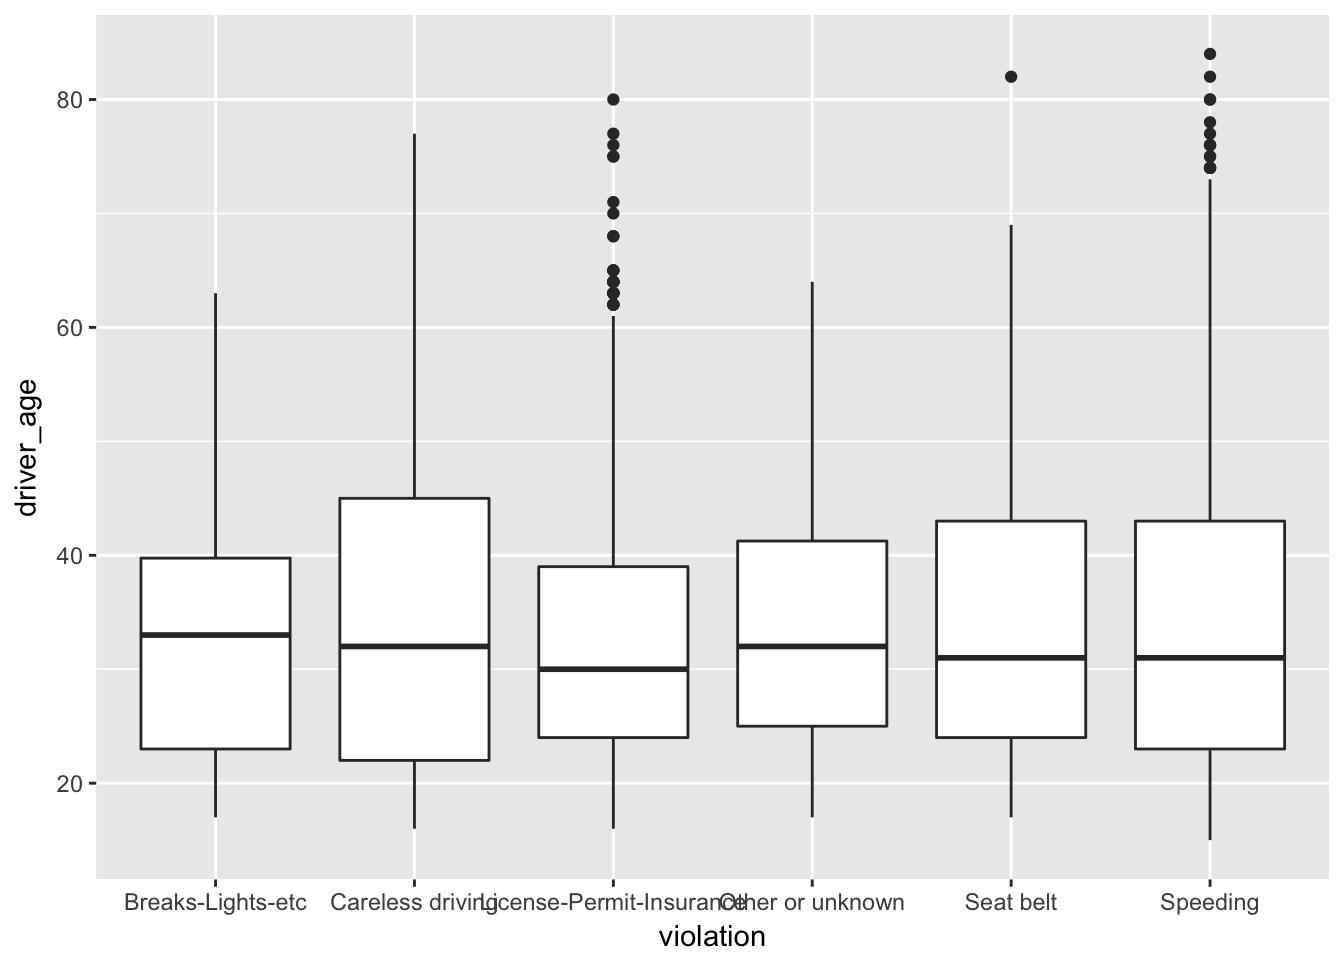
\includegraphics[width=0.7\linewidth]{R-data-wrangling_files/figure-latex/boxplot-1}

By adding points to boxplot, we can have a better idea of the number of
measurements and of their distribution.

\begin{Shaded}
\begin{Highlighting}[]
\KeywordTok{ggplot}\NormalTok{(}\DataTypeTok{data =}\NormalTok{ Chickasaw_stops, }\KeywordTok{aes}\NormalTok{(}\DataTypeTok{x =}\NormalTok{ violation, }\DataTypeTok{y =}\NormalTok{ driver_age)) }\OperatorTok{+}
\StringTok{    }\KeywordTok{geom_boxplot}\NormalTok{() }\OperatorTok{+}
\StringTok{    }\KeywordTok{geom_jitter}\NormalTok{()}
\end{Highlighting}
\end{Shaded}

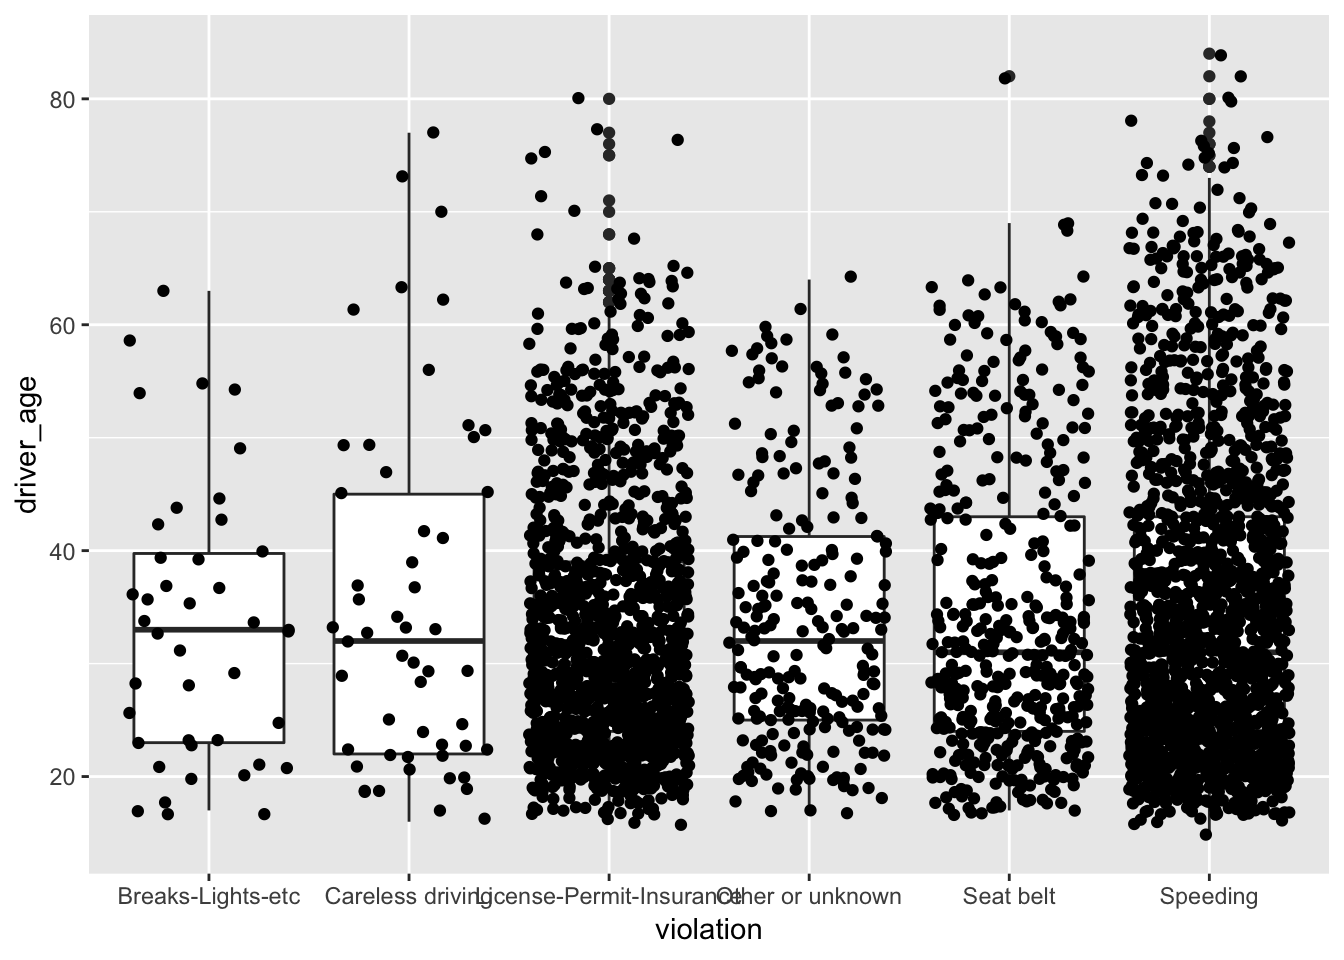
\includegraphics[width=0.7\linewidth]{R-data-wrangling_files/figure-latex/boxplot-with-jitter-1}

That looks quite messy. Let's clean it up by using the \texttt{alpha}
parameter to make the dots more transparent and also change their color:

\begin{Shaded}
\begin{Highlighting}[]
\KeywordTok{ggplot}\NormalTok{(}\DataTypeTok{data =}\NormalTok{ Chickasaw_stops, }\KeywordTok{aes}\NormalTok{(}\DataTypeTok{x =}\NormalTok{ violation, }\DataTypeTok{y =}\NormalTok{ driver_age)) }\OperatorTok{+}
\StringTok{    }\KeywordTok{geom_boxplot}\NormalTok{() }\OperatorTok{+}
\StringTok{    }\KeywordTok{geom_jitter}\NormalTok{(}\DataTypeTok{alpha =} \FloatTok{0.5}\NormalTok{, }\DataTypeTok{color =} \StringTok{"tomato"}\NormalTok{)}
\end{Highlighting}
\end{Shaded}

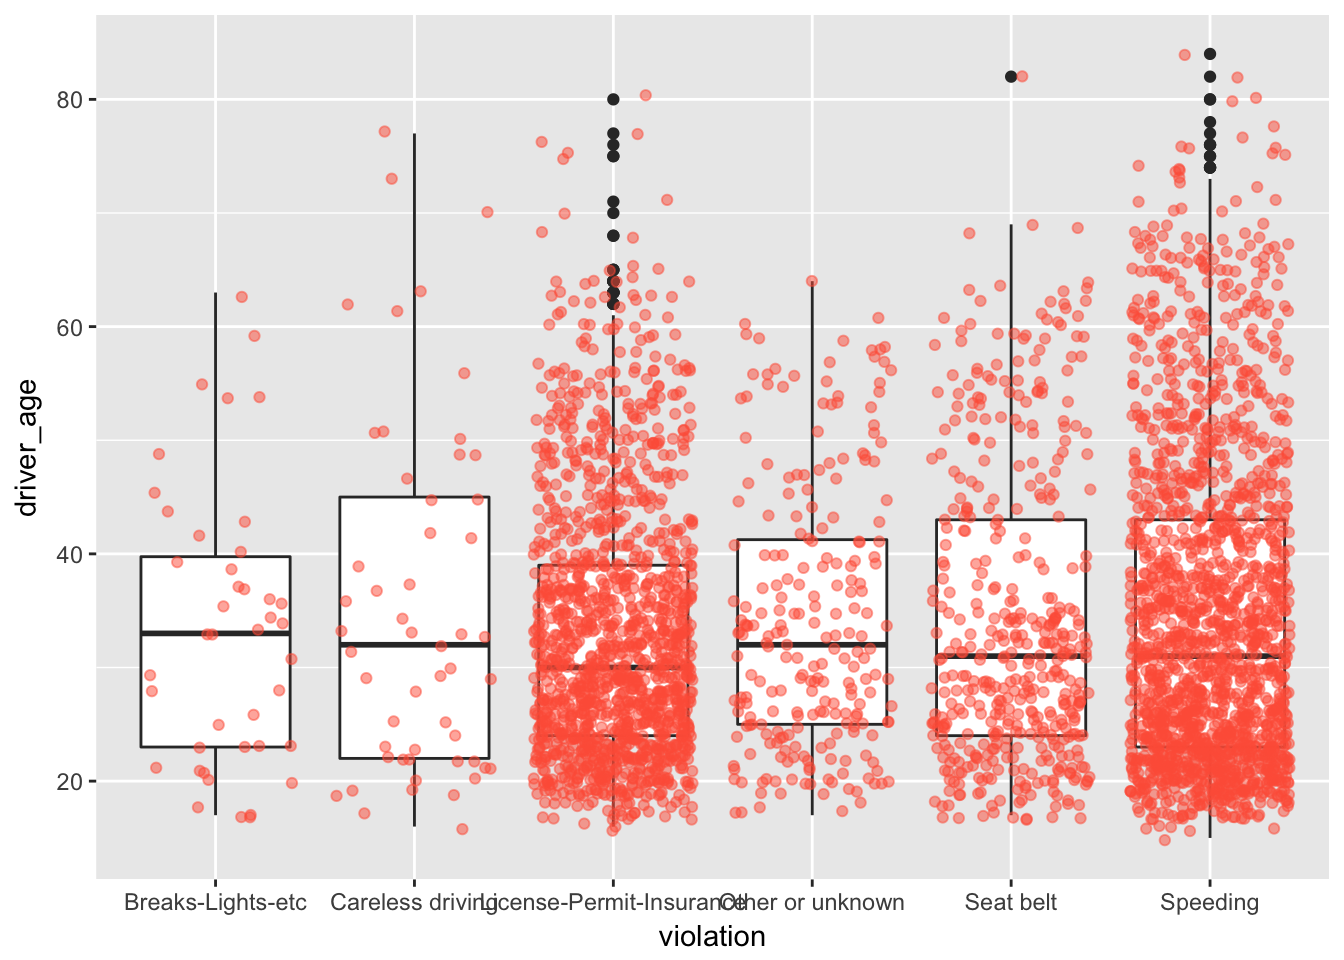
\includegraphics[width=0.7\linewidth]{R-data-wrangling_files/figure-latex/boxplot-with-jitter-transparent-1}

Notice how the boxplot layer is behind the jitter layer. We will change
the plotting order to keep the boxplot visible.

\begin{Shaded}
\begin{Highlighting}[]
\KeywordTok{ggplot}\NormalTok{(}\DataTypeTok{data =}\NormalTok{ Chickasaw_stops, }\KeywordTok{aes}\NormalTok{(}\DataTypeTok{x =}\NormalTok{ violation, }\DataTypeTok{y =}\NormalTok{ driver_age)) }\OperatorTok{+}
\StringTok{    }\KeywordTok{geom_jitter}\NormalTok{(}\DataTypeTok{alpha =} \FloatTok{0.1}\NormalTok{, }\DataTypeTok{color =} \StringTok{"tomato"}\NormalTok{) }\OperatorTok{+}\StringTok{ }
\StringTok{    }\KeywordTok{geom_boxplot}\NormalTok{()}
\end{Highlighting}
\end{Shaded}

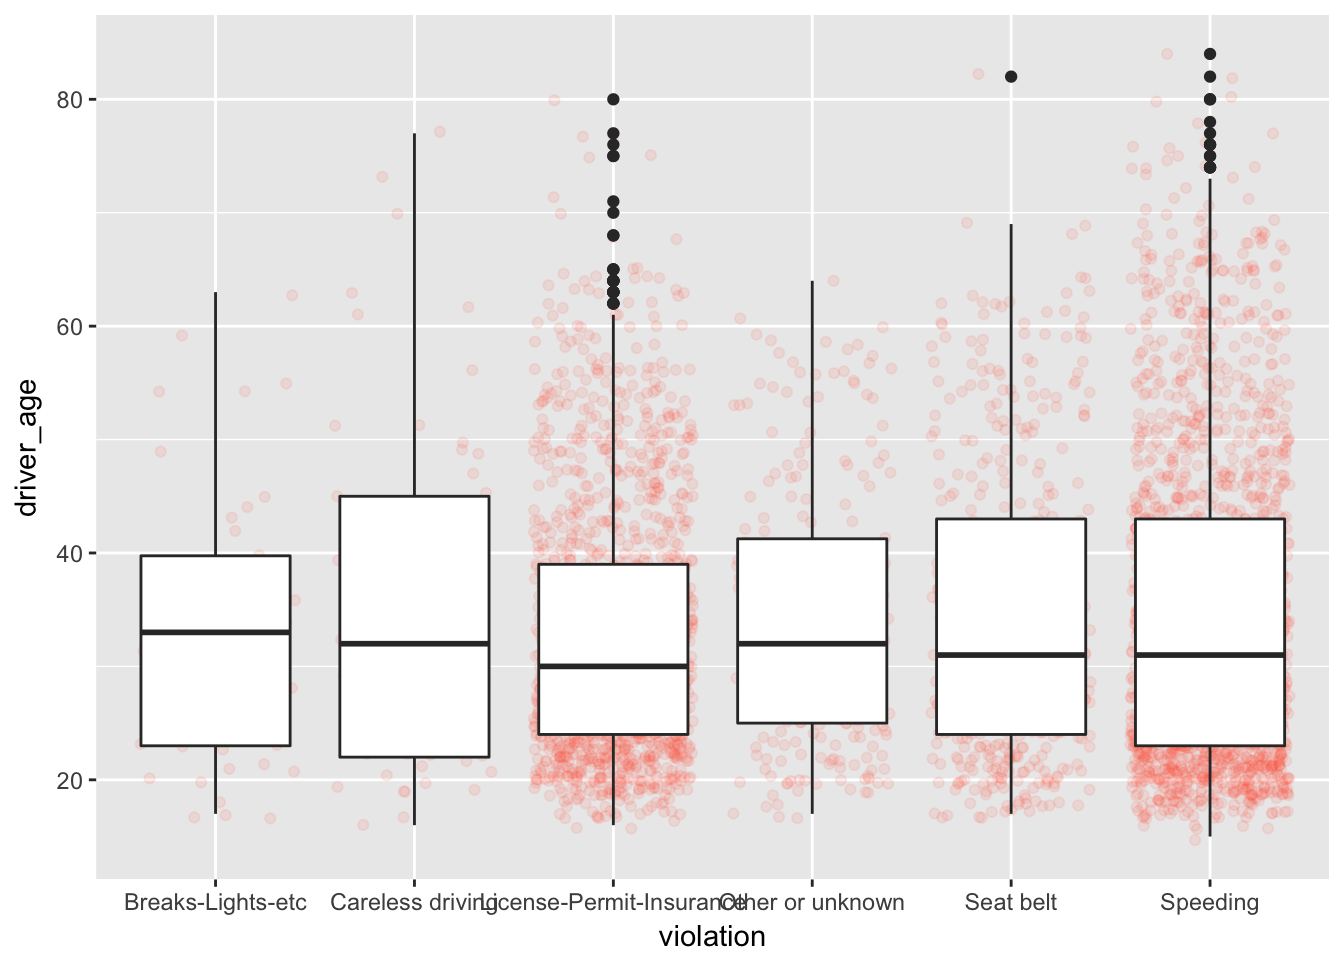
\includegraphics[width=0.7\linewidth]{R-data-wrangling_files/figure-latex/boxplot-with-jitter-reordered-1}

And finally we will change the transparency of the box plot so it does
not cover the points:

\begin{Shaded}
\begin{Highlighting}[]
\KeywordTok{ggplot}\NormalTok{(}\DataTypeTok{data =}\NormalTok{ Chickasaw_stops, }\KeywordTok{aes}\NormalTok{(}\DataTypeTok{x =}\NormalTok{ violation, }\DataTypeTok{y =}\NormalTok{ driver_age)) }\OperatorTok{+}
\StringTok{    }\KeywordTok{geom_jitter}\NormalTok{(}\DataTypeTok{alpha =} \FloatTok{0.1}\NormalTok{, }\DataTypeTok{color =} \StringTok{"tomato"}\NormalTok{) }\OperatorTok{+}
\StringTok{    }\KeywordTok{geom_boxplot}\NormalTok{(}\DataTypeTok{alpha =} \DecValTok{0}\NormalTok{)  }
\end{Highlighting}
\end{Shaded}

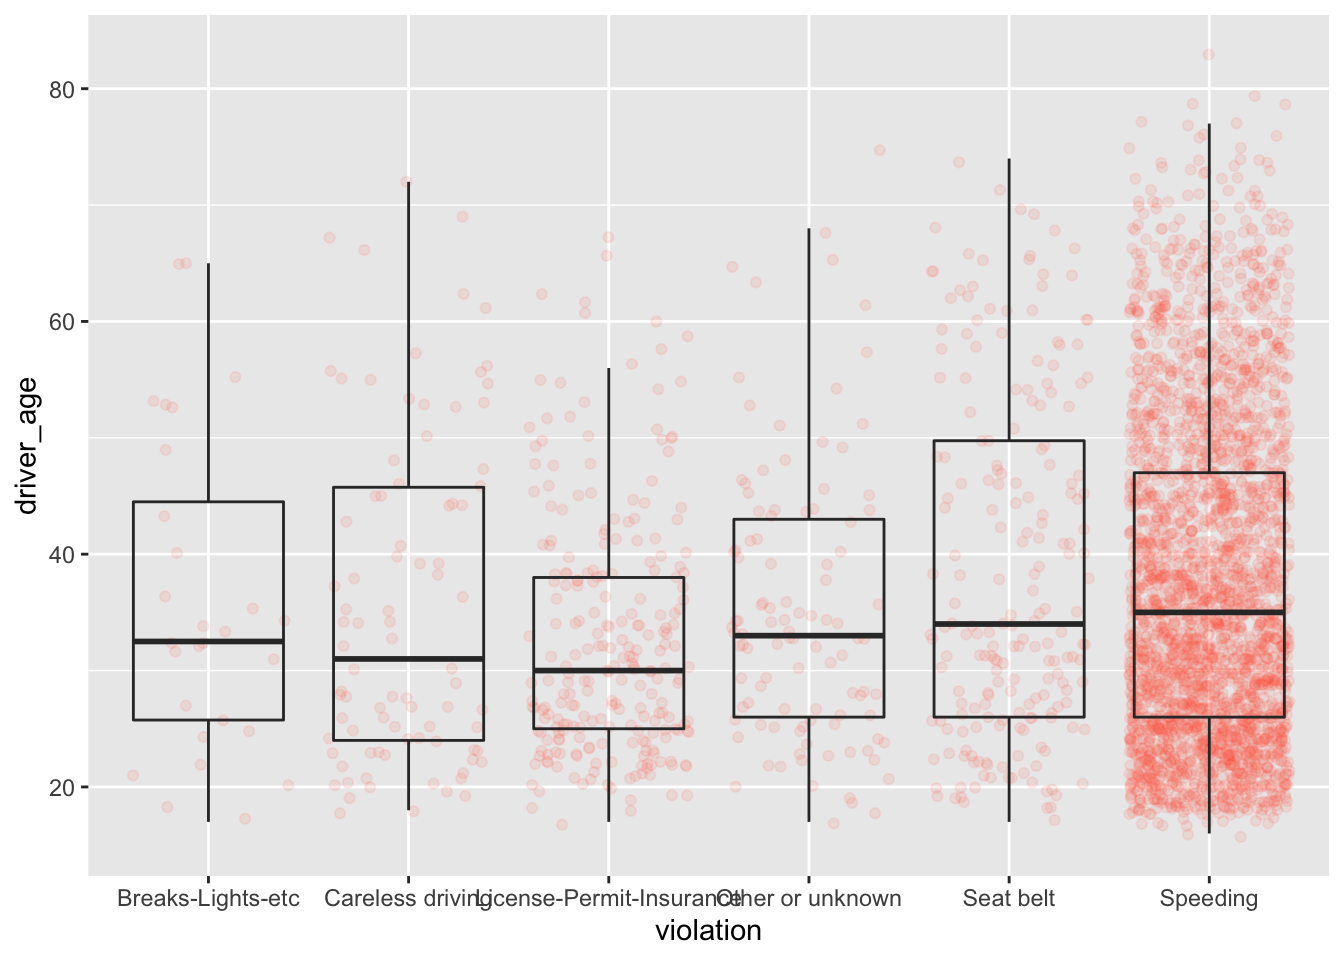
\includegraphics[width=0.7\linewidth]{R-data-wrangling_files/figure-latex/boxplot-with-jitter-clean-1}

\begin{quote}
Challenge

Boxplots are useful summaries, but hide the \emph{shape} of the
distribution. For example, if there is a bimodal distribution, it would
not be observed with a boxplot. An alternative to the boxplot is the
violin plot (sometimes known as a beanplot), where the shape (of the
density of points) is drawn.

\begin{itemize}
\tightlist
\item
  Replace the box plot with a violin plot; see \texttt{geom\_violin()}.
\end{itemize}

So far, we've looked at the distribution of age within violations Try
making a new plot to explore the distribution of age for another
variable:

\begin{itemize}
\tightlist
\item
  Create the age box plot for \texttt{driver\_race}. Overlay the boxplot
  layer on a jitter layer to show actual measurements.
\end{itemize}
\end{quote}

\section{Plotting time series data}\label{plotting-time-series-data}

To make things a little easer we first convert the date column we plan
to use to Date format.

\begin{Shaded}
\begin{Highlighting}[]
\KeywordTok{library}\NormalTok{(lubridate)}
\KeywordTok{class}\NormalTok{(trafficstops}\OperatorTok{$}\NormalTok{stop_date)}
\NormalTok{trafficstops}\OperatorTok{$}\NormalTok{stop_date <-}\StringTok{ }\KeywordTok{ymd}\NormalTok{(trafficstops}\OperatorTok{$}\NormalTok{stop_date)}
\KeywordTok{class}\NormalTok{(trafficstops}\OperatorTok{$}\NormalTok{stop_date)}
\end{Highlighting}
\end{Shaded}

Let's calculate number of violation per weekday. For better
understanding we will label the weekdays. First we need to group the
data and count records within each group:

\begin{Shaded}
\begin{Highlighting}[]
\NormalTok{trafficstops }\OperatorTok\StringTok{ }
\StringTok{  }\KeywordTok{mutate}\NormalTok{(}\DataTypeTok{wk_day =} \KeywordTok{wday}\NormalTok{(stop_date, }\DataTypeTok{label =} \OtherTok{TRUE}\NormalTok{)) }\OperatorTok\StringTok{  }
\StringTok{  }\KeywordTok{group_by}\NormalTok{(wk_day, violation) }\OperatorTok
\StringTok{  }\NormalTok{tally}
\end{Highlighting}
\end{Shaded}

Timelapse data can be visualized as a line plot (with -- you guessed it
-- \texttt{geom\_line()}) mapping the days to the x axis and counts to
the y axis. So we pipe the output from above into ggplot like this:

\begin{Shaded}
\begin{Highlighting}[]
\NormalTok{trafficstops }\OperatorTok\StringTok{ }
\StringTok{  }\KeywordTok{mutate}\NormalTok{(}\DataTypeTok{wk_day =} \KeywordTok{wday}\NormalTok{(stop_date, }\DataTypeTok{label =} \OtherTok{TRUE}\NormalTok{)) }\OperatorTok\StringTok{  }
\StringTok{  }\KeywordTok{group_by}\NormalTok{(wk_day, violation) }\OperatorTok
\StringTok{  }\NormalTok{tally }\OperatorTok\StringTok{ }
\StringTok{  }\KeywordTok{ggplot}\NormalTok{(}\KeywordTok{aes}\NormalTok{(}\DataTypeTok{x =}\NormalTok{ wk_day, }\DataTypeTok{y =}\NormalTok{ n)) }\OperatorTok{+}
\StringTok{     }\KeywordTok{geom_line}\NormalTok{()}
\end{Highlighting}
\end{Shaded}

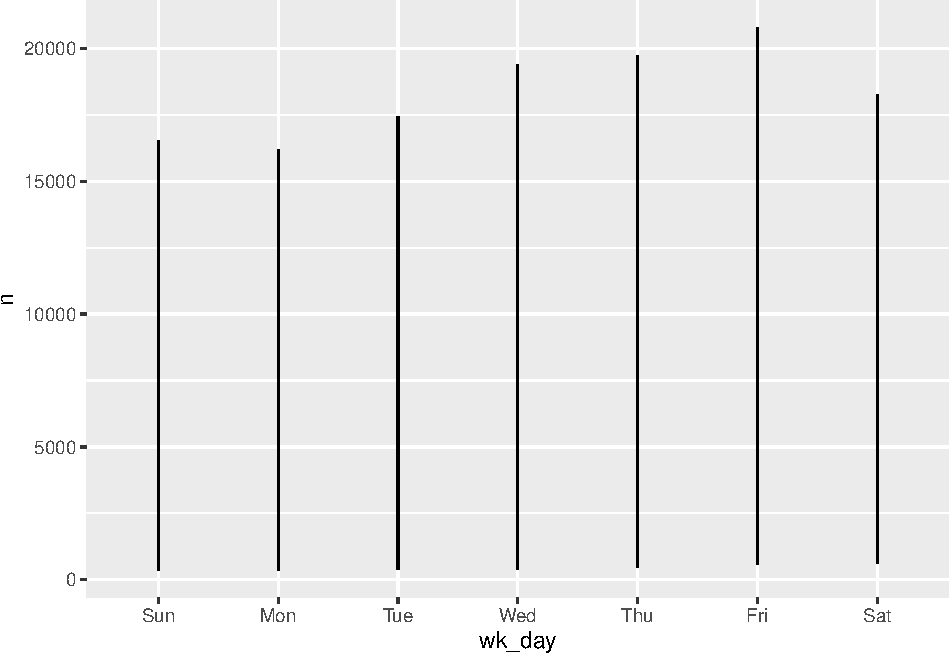
\includegraphics{R-data-wrangling_files/figure-latex/first-time-series-1.pdf}

Unfortunately, this does not work because we plotted data for all the
violations together. So what ggplot displays is the range of all values
for each year in a vertial line. We need to tell ggplot to draw a line
for each violation by modifying the aesthetic function to include
\texttt{group\ =\ violation}:

\begin{Shaded}
\begin{Highlighting}[]
\NormalTok{trafficstops }\OperatorTok\StringTok{ }
\StringTok{  }\KeywordTok{mutate}\NormalTok{(}\DataTypeTok{wk_day =} \KeywordTok{wday}\NormalTok{(stop_date, }\DataTypeTok{label =} \OtherTok{TRUE}\NormalTok{)) }\OperatorTok\StringTok{  }
\StringTok{  }\KeywordTok{group_by}\NormalTok{(wk_day, violation) }\OperatorTok
\StringTok{  }\NormalTok{tally }\OperatorTok\StringTok{ }
\StringTok{  }\KeywordTok{ggplot}\NormalTok{(}\KeywordTok{aes}\NormalTok{(}\DataTypeTok{x =}\NormalTok{ wk_day, }\DataTypeTok{y =}\NormalTok{ n, }\DataTypeTok{group =}\NormalTok{ violation)) }\OperatorTok{+}
\StringTok{     }\KeywordTok{geom_line}\NormalTok{()}
\end{Highlighting}
\end{Shaded}

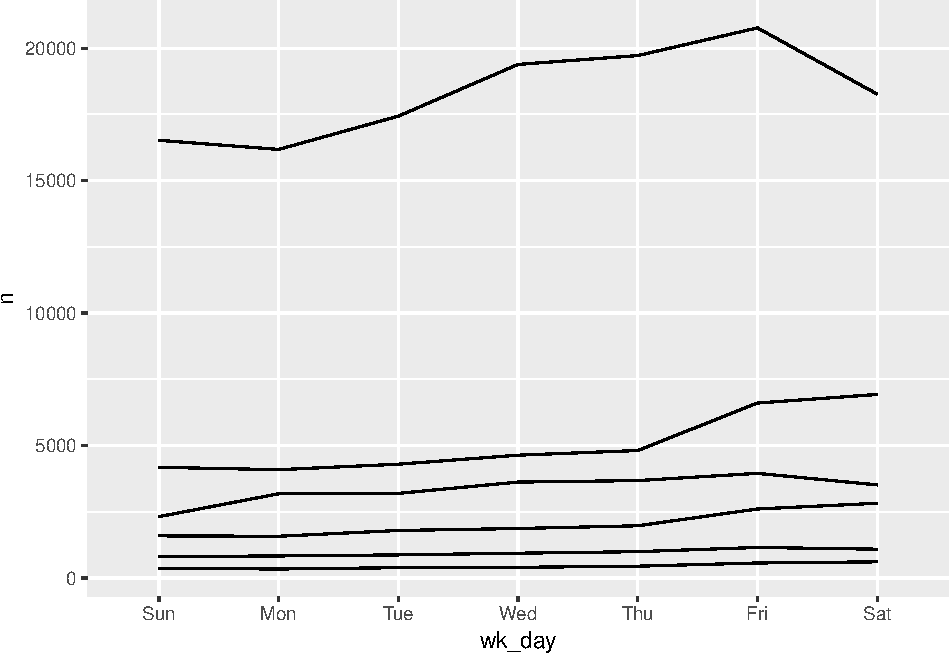
\includegraphics[width=0.7\linewidth]{R-data-wrangling_files/figure-latex/time-series-by-violation-1}

We will be able to distinguish violations in the plot if we add colors.
(Colors groups automatically if the variable is numeric).

\begin{Shaded}
\begin{Highlighting}[]
\NormalTok{trafficstops }\OperatorTok\StringTok{ }
\StringTok{  }\KeywordTok{mutate}\NormalTok{(}\DataTypeTok{wk_day =} \KeywordTok{wday}\NormalTok{(stop_date, }\DataTypeTok{label =} \OtherTok{TRUE}\NormalTok{)) }\OperatorTok\StringTok{  }
\StringTok{  }\KeywordTok{group_by}\NormalTok{(wk_day, violation) }\OperatorTok
\StringTok{  }\NormalTok{tally }\OperatorTok\StringTok{ }
\StringTok{  }\KeywordTok{ggplot}\NormalTok{(}\KeywordTok{aes}\NormalTok{(}\DataTypeTok{x =}\NormalTok{ wk_day, }\DataTypeTok{y =}\NormalTok{ n, }\DataTypeTok{group =}\NormalTok{ violation, }\DataTypeTok{color =}\NormalTok{ violation)) }\OperatorTok{+}
\StringTok{     }\KeywordTok{geom_line}\NormalTok{()}
\end{Highlighting}
\end{Shaded}

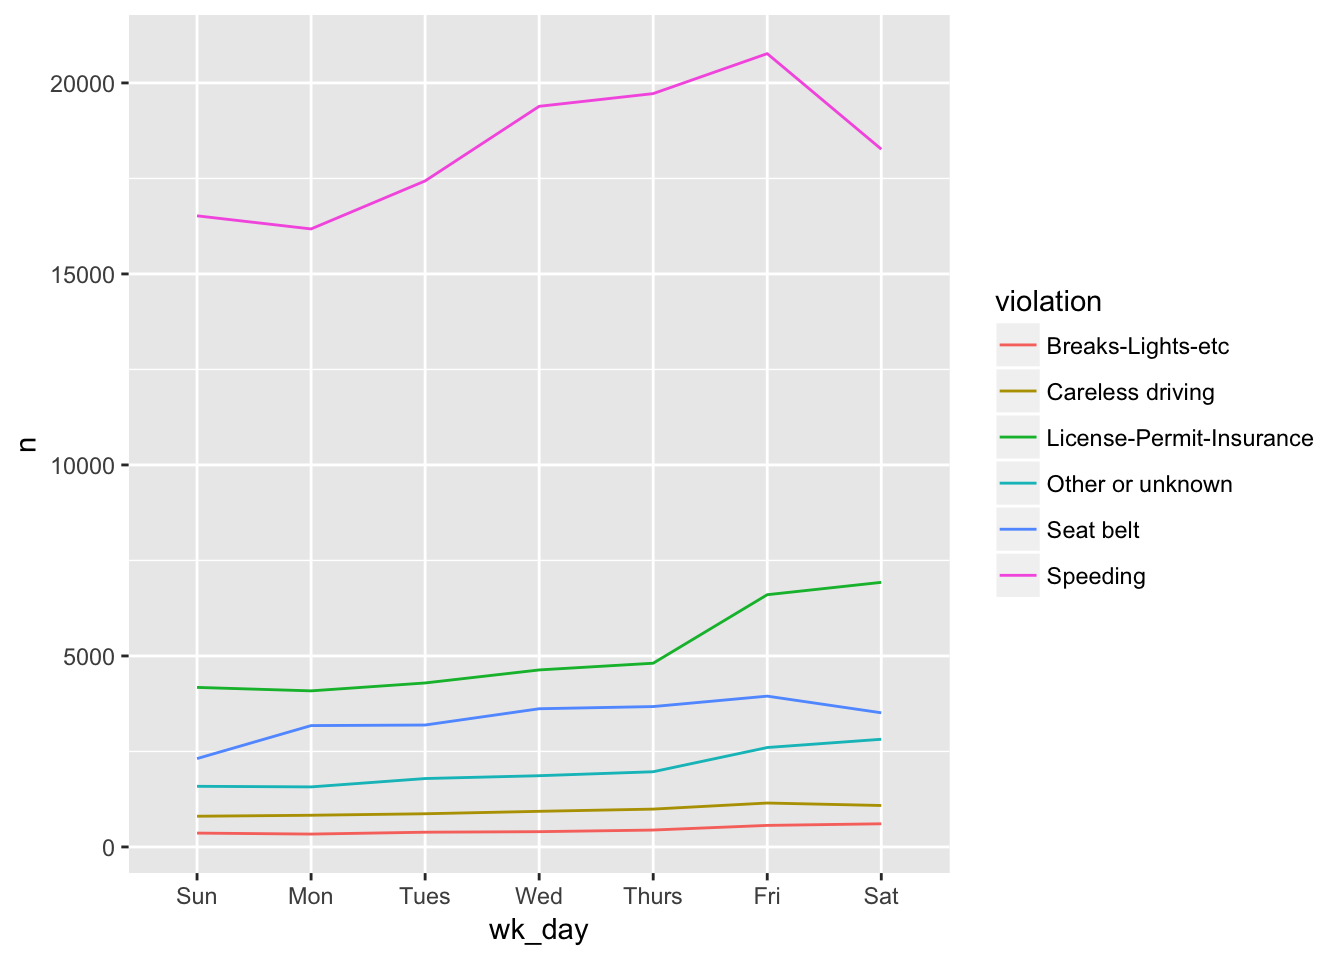
\includegraphics[width=0.7\linewidth]{R-data-wrangling_files/figure-latex/time-series-with-colors-1}

\section{Faceting}\label{faceting}

ggplot has a special technique called \emph{faceting} that allows to
split one plot into multiple plots based on a factor included in the
dataset. We will use it to make a time series plot for each violation:

\begin{Shaded}
\begin{Highlighting}[]
\NormalTok{trafficstops }\OperatorTok\StringTok{ }
\StringTok{  }\KeywordTok{mutate}\NormalTok{(}\DataTypeTok{wk_day =} \KeywordTok{wday}\NormalTok{(stop_date, }\DataTypeTok{label =} \OtherTok{TRUE}\NormalTok{)) }\OperatorTok\StringTok{  }
\StringTok{  }\KeywordTok{group_by}\NormalTok{(wk_day, violation) }\OperatorTok
\StringTok{  }\NormalTok{tally }\OperatorTok\StringTok{ }
\StringTok{  }\KeywordTok{ggplot}\NormalTok{(}\KeywordTok{aes}\NormalTok{(}\DataTypeTok{x =}\NormalTok{ wk_day, }\DataTypeTok{y =}\NormalTok{ n, }\DataTypeTok{group =}\NormalTok{ violation)) }\OperatorTok{+}
\StringTok{     }\KeywordTok{geom_line}\NormalTok{() }\OperatorTok{+}
\StringTok{     }\KeywordTok{facet_wrap}\NormalTok{(}\OperatorTok{~}\StringTok{ }\NormalTok{violation)}
\end{Highlighting}
\end{Shaded}

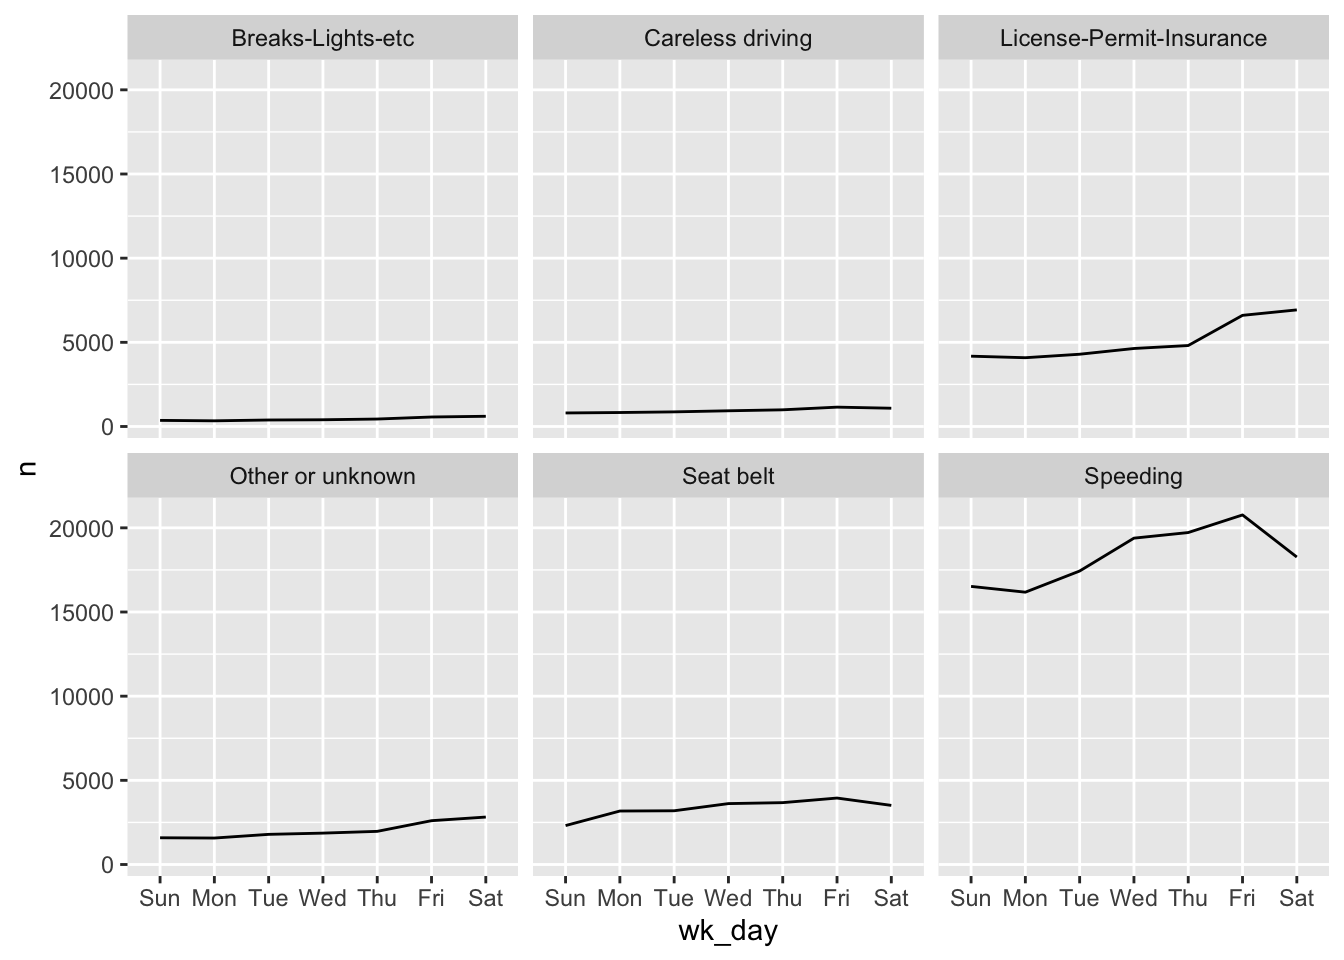
\includegraphics[width=0.7\linewidth]{R-data-wrangling_files/figure-latex/first-facet-1}

Now we would like to split the line in each plot by the race of the
driver. To do that we need to make counts in the data frame grouped by
\texttt{day}, \texttt{violation}, and \texttt{driver\_race}. We then
make the faceted plot by splitting further by race using \texttt{color}
and \texttt{group} (within a single plot):

\begin{Shaded}
\begin{Highlighting}[]
\NormalTok{trafficstops }\OperatorTok\StringTok{ }
\StringTok{  }\KeywordTok{mutate}\NormalTok{(}\DataTypeTok{wk_day =} \KeywordTok{wday}\NormalTok{(stop_date, }\DataTypeTok{label=}\OtherTok{TRUE}\NormalTok{)) }\OperatorTok\StringTok{ }
\StringTok{  }\KeywordTok{group_by}\NormalTok{(wk_day, violation, driver_race) }\OperatorTok
\StringTok{  }\NormalTok{tally }\OperatorTok\StringTok{ }
\StringTok{  }\KeywordTok{ggplot}\NormalTok{(}\KeywordTok{aes}\NormalTok{(}\DataTypeTok{x =}\NormalTok{ wk_day, }\DataTypeTok{y =}\NormalTok{ n, }\DataTypeTok{color =}\NormalTok{ driver_race, }\DataTypeTok{group =}\NormalTok{ driver_race)) }\OperatorTok{+}
\StringTok{  }\KeywordTok{geom_line}\NormalTok{() }\OperatorTok{+}\StringTok{ }
\StringTok{  }\KeywordTok{facet_wrap}\NormalTok{(}\OperatorTok{~}\StringTok{ }\NormalTok{violation)}
\end{Highlighting}
\end{Shaded}

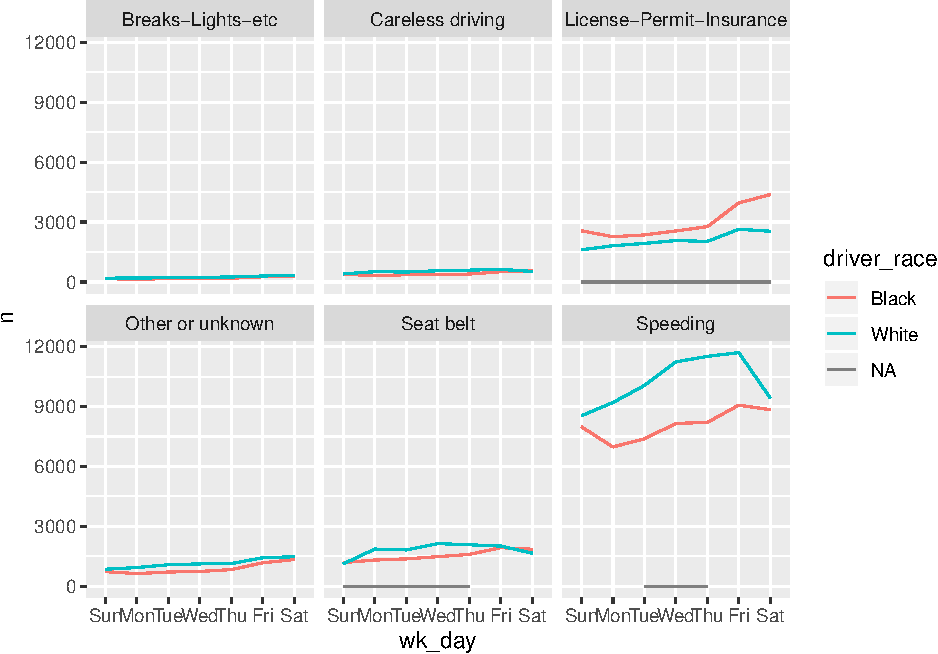
\includegraphics{R-data-wrangling_files/figure-latex/facet-by-violation-and-race-1.pdf}

Note that there is an alternative, the \texttt{facet\_grid} geometry,
which allows you to explicitly specify how you want your plots to be
arranged via formula notation
(\texttt{rows\ \textasciitilde{}\ columns}; a \texttt{.} can be used as
a placeholder that indicates only one row or column).

\begin{quote}
Challenge

Use what you just learned to create a plot that depicts how the average
age of each driver for the two recorded ethnicities changes through the
week. Hint: make sure you remove the records with driver\_age under 16.
How would you go about visualizing both lines and points on the plot?
How would you split your plot into one per each violation type?
\end{quote}

\section{\texorpdfstring{\textbf{\texttt{ggplot2}}
themes}{ggplot2 themes}}\label{ggplot2-themes}

\textbf{\texttt{ggplot2}} comes with several other themes which can be
useful to quickly change the look of your visualization, for example
\texttt{theme\_bw()} changes the plot background to white:

\begin{Shaded}
\begin{Highlighting}[]
\NormalTok{trafficstops }\OperatorTok\StringTok{ }
\StringTok{  }\KeywordTok{mutate}\NormalTok{(}\DataTypeTok{wk_day =} \KeywordTok{wday}\NormalTok{(stop_date, }\DataTypeTok{label=}\OtherTok{TRUE}\NormalTok{, }\DataTypeTok{abbr=}\OtherTok{TRUE}\NormalTok{)) }\OperatorTok\StringTok{ }
\StringTok{  }\KeywordTok{group_by}\NormalTok{(wk_day, violation, driver_race) }\OperatorTok
\StringTok{  }\NormalTok{tally }\OperatorTok\StringTok{ }
\StringTok{  }\KeywordTok{ggplot}\NormalTok{(}\KeywordTok{aes}\NormalTok{(}\DataTypeTok{x =}\NormalTok{ wk_day, }\DataTypeTok{y =}\NormalTok{ n, }\DataTypeTok{color =}\NormalTok{ driver_race, }\DataTypeTok{group =}\NormalTok{ driver_race)) }\OperatorTok{+}
\StringTok{  }\KeywordTok{geom_line}\NormalTok{() }\OperatorTok{+}\StringTok{ }
\StringTok{  }\KeywordTok{facet_wrap}\NormalTok{(}\OperatorTok{~}\StringTok{ }\NormalTok{violation) }\OperatorTok{+}
\StringTok{  }\KeywordTok{theme_bw}\NormalTok{()}
\end{Highlighting}
\end{Shaded}

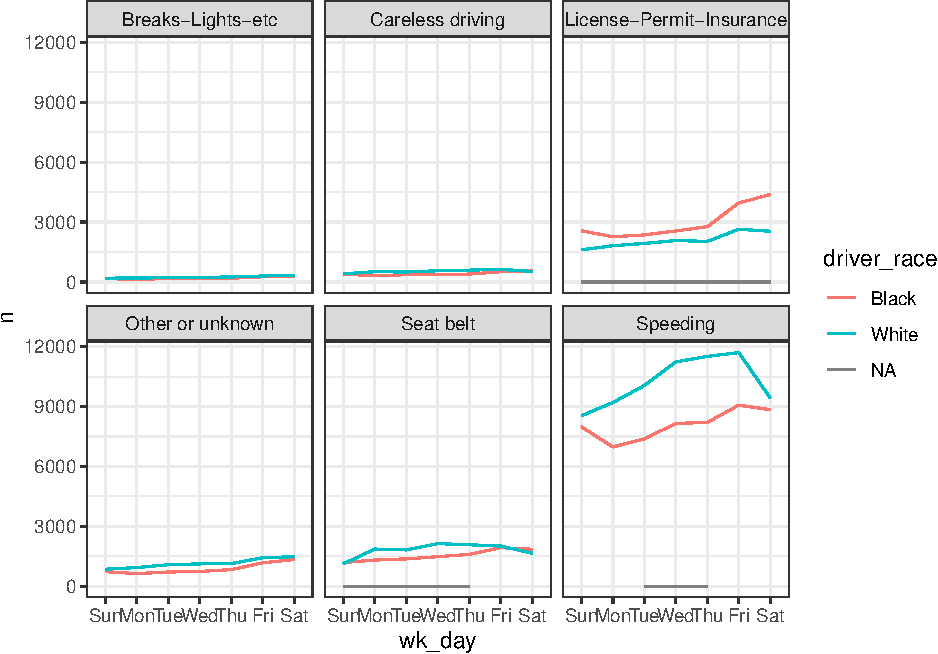
\includegraphics{R-data-wrangling_files/figure-latex/facet-theming-1.pdf}

The complete list of themes is available at
\url{http://docs.ggplot2.org/current/ggtheme.html}.
\texttt{theme\_minimal()} and \texttt{theme\_light()} are popular, and
\texttt{theme\_void()} can be useful as a starting point to create a new
hand-crafted theme.

The
\href{https://cran.r-project.org/web/packages/ggthemes/vignettes/ggthemes.html}{ggthemes}
package provides a wide variety of options (including an Excel 2003
theme). The
\href{https://www.ggplot2-exts.org}{\textbf{\texttt{ggplot2}} extensions
website} provides a list of packages that extend the capabilities of
\textbf{\texttt{ggplot2}}, including additional themes.

\section{Customization}\label{customization}

There are endless possibilities to customize your plot, particularly
when you are ready for publication or presentation. Let's look into just
a few examples. Before we do that we will assign our plot above to a
variable.

\begin{Shaded}
\begin{Highlighting}[]
\NormalTok{stops_facet_plot <-}\StringTok{ }\NormalTok{trafficstops }\OperatorTok\StringTok{ }
\StringTok{  }\KeywordTok{mutate}\NormalTok{(}\DataTypeTok{wk_day =} \KeywordTok{wday}\NormalTok{(stop_date, }\DataTypeTok{label=}\OtherTok{TRUE}\NormalTok{, }\DataTypeTok{abbr=}\OtherTok{TRUE}\NormalTok{)) }\OperatorTok\StringTok{ }
\StringTok{  }\KeywordTok{group_by}\NormalTok{(wk_day, violation, driver_race) }\OperatorTok
\StringTok{  }\NormalTok{tally }\OperatorTok\StringTok{ }
\StringTok{  }\KeywordTok{ggplot}\NormalTok{(}\KeywordTok{aes}\NormalTok{(}\DataTypeTok{x =}\NormalTok{ wk_day, }\DataTypeTok{y =}\NormalTok{ n, }\DataTypeTok{color =}\NormalTok{ driver_race, }\DataTypeTok{group =}\NormalTok{ driver_race)) }\OperatorTok{+}
\StringTok{  }\KeywordTok{geom_line}\NormalTok{() }\OperatorTok{+}\StringTok{ }
\StringTok{  }\KeywordTok{facet_wrap}\NormalTok{(}\OperatorTok{~}\StringTok{ }\NormalTok{violation)}
\end{Highlighting}
\end{Shaded}

Now, let's change names of axes to something more informative than
`wk\_day' and `n' and add a title to the figure:

\begin{Shaded}
\begin{Highlighting}[]
\NormalTok{stops_facet_plot }\OperatorTok{+}
\StringTok{  }\KeywordTok{labs}\NormalTok{(}\DataTypeTok{title =} \StringTok{'Observed violations per day of week'}\NormalTok{,}
         \DataTypeTok{x =} \StringTok{'Weekday of observation'}\NormalTok{,}
         \DataTypeTok{y =} \StringTok{'Number of violations'}\NormalTok{) }\OperatorTok{+}
\StringTok{  }\KeywordTok{theme_bw}\NormalTok{()}
\end{Highlighting}
\end{Shaded}

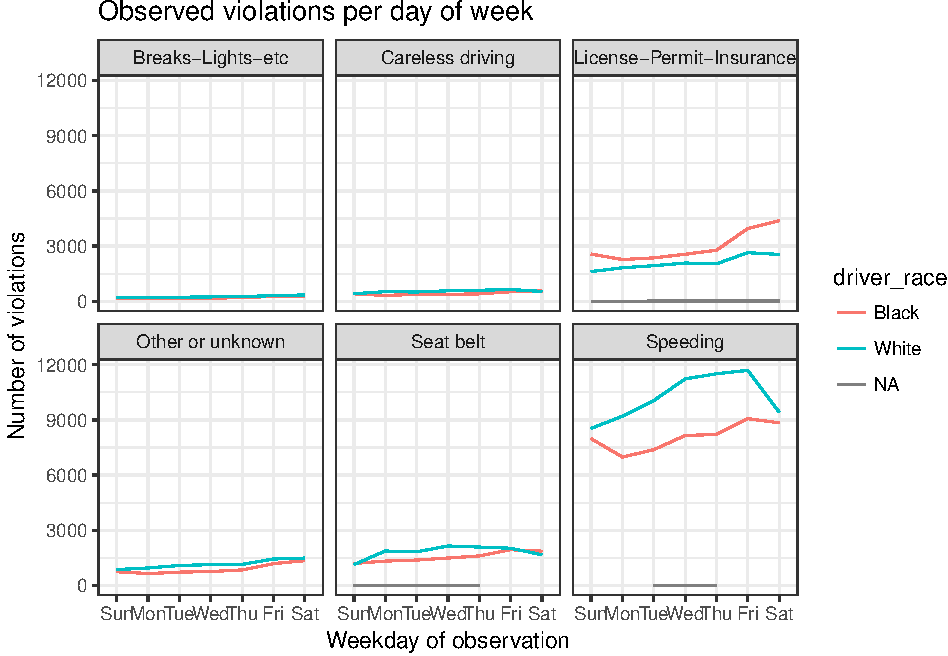
\includegraphics{R-data-wrangling_files/figure-latex/improved-labels-1.pdf}

The axes have more informative names, but their readability can be
improved by increasing the font size:

\begin{Shaded}
\begin{Highlighting}[]
\NormalTok{stops_facet_plot }\OperatorTok{+}
\StringTok{  }\KeywordTok{labs}\NormalTok{(}\DataTypeTok{title =} \StringTok{'Observed violations per day of week'}\NormalTok{,}
         \DataTypeTok{x =} \StringTok{'Weekday of observation'}\NormalTok{,}
         \DataTypeTok{y =} \StringTok{'Number of violations'}\NormalTok{) }\OperatorTok{+}
\StringTok{  }\KeywordTok{theme_bw}\NormalTok{() }\OperatorTok{+}\StringTok{ }
\StringTok{  }\KeywordTok{theme}\NormalTok{(}\DataTypeTok{text =} \KeywordTok{element_text}\NormalTok{(}\DataTypeTok{size=}\DecValTok{16}\NormalTok{))}
\end{Highlighting}
\end{Shaded}

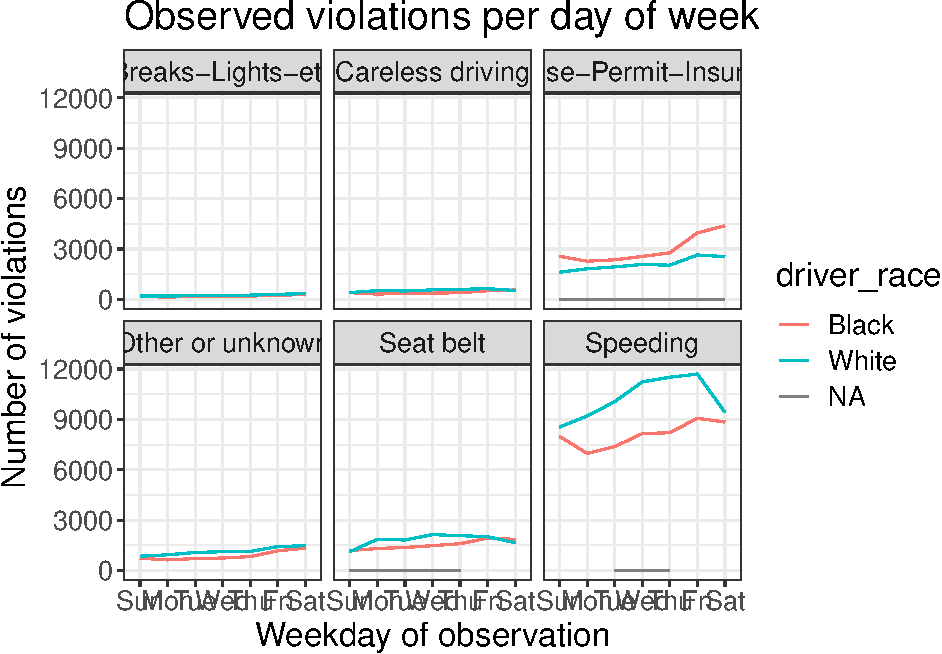
\includegraphics{R-data-wrangling_files/figure-latex/improved-font-size-1.pdf}

After our manipulations, you may notice that the values on the x-axis
are still not properly readable. Let's change the orientation of the
labels and adjust them vertically and horizontally so they don't
overlap. You can use a 90 degree angle, or experiment to find the
appropriate angle for diagonally oriented labels:

\begin{Shaded}
\begin{Highlighting}[]
\NormalTok{stops_facet_plot }\OperatorTok{+}
\StringTok{  }\KeywordTok{labs}\NormalTok{(}\DataTypeTok{title =} \StringTok{'Observed violations per day of week'}\NormalTok{,}
         \DataTypeTok{x =} \StringTok{'Weekday of observation'}\NormalTok{,}
         \DataTypeTok{y =} \StringTok{'Number of violations'}\NormalTok{) }\OperatorTok{+}
\StringTok{  }\KeywordTok{theme_bw}\NormalTok{() }\OperatorTok{+}\StringTok{ }
\StringTok{  }\KeywordTok{theme}\NormalTok{(}\DataTypeTok{axis.text.x =} \KeywordTok{element_text}\NormalTok{(}\DataTypeTok{colour=}\StringTok{"grey40"}\NormalTok{, }\DataTypeTok{size=}\DecValTok{12}\NormalTok{, }\DataTypeTok{angle=}\DecValTok{90}\NormalTok{, }\DataTypeTok{hjust=}\NormalTok{.}\DecValTok{5}\NormalTok{, }\DataTypeTok{vjust=}\NormalTok{.}\DecValTok{5}\NormalTok{),}
        \DataTypeTok{axis.text.y =} \KeywordTok{element_text}\NormalTok{(}\DataTypeTok{colour=}\StringTok{"grey40"}\NormalTok{, }\DataTypeTok{size=}\DecValTok{12}\NormalTok{),}
        \DataTypeTok{strip.text =} \KeywordTok{element_text}\NormalTok{(}\DataTypeTok{size=}\DecValTok{14}\NormalTok{),}
        \DataTypeTok{text =} \KeywordTok{element_text}\NormalTok{(}\DataTypeTok{size=}\DecValTok{16}\NormalTok{))}
\end{Highlighting}
\end{Shaded}

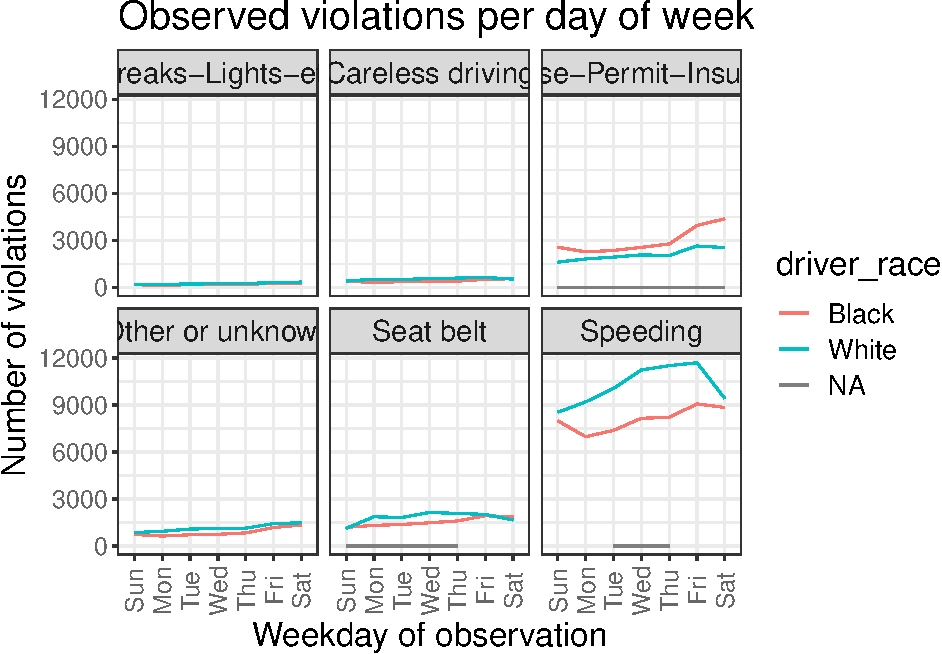
\includegraphics{R-data-wrangling_files/figure-latex/tilted-xlabels-1.pdf}

If you like the changes you created better than the default theme, you
can save them as an object to be able to easily apply them to other
plots you may create:

\begin{Shaded}
\begin{Highlighting}[]
\NormalTok{grey_theme <-}\StringTok{ }\KeywordTok{theme}\NormalTok{(}\DataTypeTok{axis.text.x =} \KeywordTok{element_text}\NormalTok{(}\DataTypeTok{colour=}\StringTok{"grey40"}\NormalTok{, }\DataTypeTok{size=}\DecValTok{12}\NormalTok{, }\DataTypeTok{angle=}\DecValTok{90}\NormalTok{, }\DataTypeTok{hjust=}\NormalTok{.}\DecValTok{5}\NormalTok{, }\DataTypeTok{vjust=}\NormalTok{.}\DecValTok{5}\NormalTok{),}
                   \DataTypeTok{axis.text.y =} \KeywordTok{element_text}\NormalTok{(}\DataTypeTok{colour=}\StringTok{"grey40"}\NormalTok{, }\DataTypeTok{size=}\DecValTok{12}\NormalTok{), }\DataTypeTok{text=}\KeywordTok{element_text}\NormalTok{(}\DataTypeTok{size=}\DecValTok{16}\NormalTok{))}

\KeywordTok{ggplot}\NormalTok{(}\DataTypeTok{data =}\NormalTok{ Chickasaw_stops, }\KeywordTok{aes}\NormalTok{(}\DataTypeTok{x =}\NormalTok{ violation, }\DataTypeTok{y =}\NormalTok{ driver_age)) }\OperatorTok{+}
\StringTok{  }\KeywordTok{geom_boxplot}\NormalTok{() }\OperatorTok{+}\StringTok{ }
\StringTok{  }\NormalTok{grey_theme}
\end{Highlighting}
\end{Shaded}

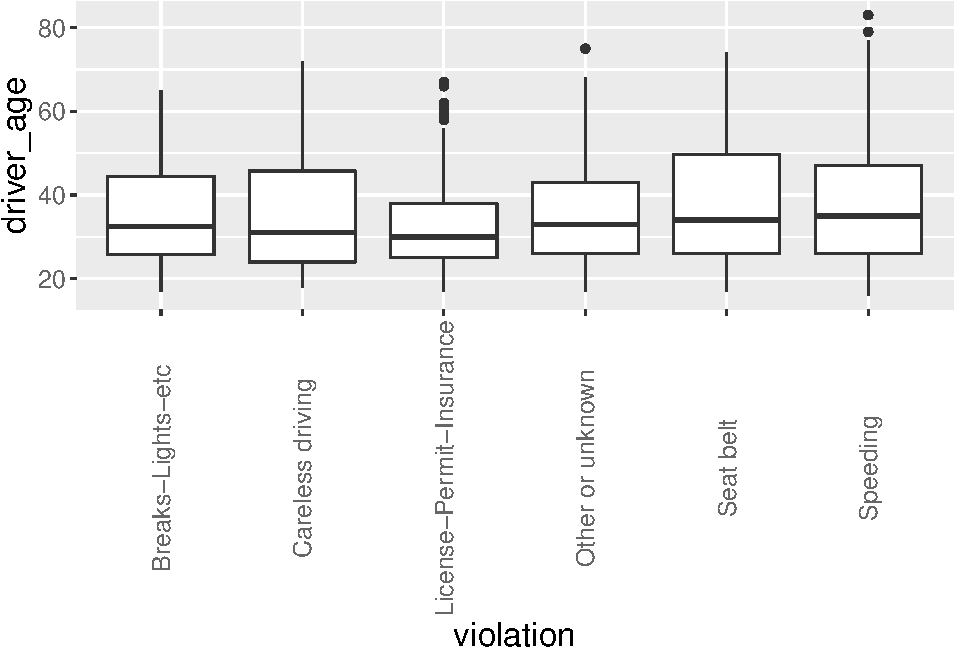
\includegraphics{R-data-wrangling_files/figure-latex/save-reapply-theme-1.pdf}

Note that it is also possible to change the fonts of your plots. If you
are on Windows, you may have to install the
\href{https://github.com/wch/extrafont}{\textbf{extrafont} package}, and
follow the instructions included in the README for this package.

\begin{quote}
Challenge

With all of this information in hand, please take another five minutes
to either improve one of the plots generated in this exercise or create
a beautiful graph of your own. Use the RStudio
\href{https://www.rstudio.com/wp-content/uploads/2016/11/ggplot2-cheatsheet-2.1.pdf}{\textbf{\texttt{ggplot2}}
cheat sheet} for inspiration.
\end{quote}

\begin{quote}
Here are some ideas:
\end{quote}

\begin{quote}
\begin{itemize}
\tightlist
\item
  See if you can change the thickness of the lines.
\item
  Can you find a way to change the name of the legend? What about its
  labels?
\item
  Try using a different color palette (see
  \url{http://www.cookbook-r.com/Graphs/Colors_(ggplot2)/}).
\end{itemize}
\end{quote}

After creating your plot, you can save it out to a file in your prefered
format. You can change the dimension (and resolution) of your plot by
adjusting the appropriate arguments (\texttt{width}, \texttt{height} and
\texttt{dpi}):

\begin{Shaded}
\begin{Highlighting}[]
\NormalTok{my_plot <-}\StringTok{ }\NormalTok{stops_facet_plot }\OperatorTok{+}
\StringTok{  }\KeywordTok{labs}\NormalTok{(}\DataTypeTok{title =} \StringTok{'Observed violations per day of week'}\NormalTok{,}
         \DataTypeTok{x =} \StringTok{'Weekday of observation'}\NormalTok{,}
         \DataTypeTok{y =} \StringTok{'Number of violations'}\NormalTok{) }\OperatorTok{+}
\StringTok{  }\KeywordTok{theme_bw}\NormalTok{() }\OperatorTok{+}\StringTok{ }
\StringTok{  }\KeywordTok{theme}\NormalTok{(}\DataTypeTok{axis.text.x =} \KeywordTok{element_text}\NormalTok{(}\DataTypeTok{colour=}\StringTok{"grey40"}\NormalTok{, }\DataTypeTok{size=}\DecValTok{12}\NormalTok{, }\DataTypeTok{angle=}\DecValTok{90}\NormalTok{, }\DataTypeTok{hjust=}\NormalTok{.}\DecValTok{5}\NormalTok{, }\DataTypeTok{vjust=}\NormalTok{.}\DecValTok{5}\NormalTok{),}
        \DataTypeTok{axis.text.y =} \KeywordTok{element_text}\NormalTok{(}\DataTypeTok{colour=}\StringTok{"grey40"}\NormalTok{, }\DataTypeTok{size=}\DecValTok{12}\NormalTok{),}
        \DataTypeTok{strip.text =} \KeywordTok{element_text}\NormalTok{(}\DataTypeTok{size=}\DecValTok{14}\NormalTok{),}
        \DataTypeTok{text =} \KeywordTok{element_text}\NormalTok{(}\DataTypeTok{size=}\DecValTok{16}\NormalTok{))}

\KeywordTok{ggsave}\NormalTok{(}\StringTok{"name_of_file.png"}\NormalTok{, my_plot, }\DataTypeTok{width=}\DecValTok{15}\NormalTok{, }\DataTypeTok{height=}\DecValTok{10}\NormalTok{)}
\end{Highlighting}
\end{Shaded}

Note: The parameters \texttt{width} and \texttt{height} also determine
the font size in the saved plot.

\bibliography{book.bib,packages.bib}


\end{document}
